\documentclass{article}

\usepackage{sdpgf}

\usepackage{amsmath,amsfonts,amssymb}

\usepackage{tikz}
\usetikzlibrary{shapes.multipart,calc}


\newcommand{\N}{\mathbb{N}}
\newcommand{\Z}{\mathbb{Z}}


\usepackage{amsthm}

% \newtheorem{theorem}{Theorem}
% \newtheorem{lemma}[theorem]{Lemma}
% \newtheorem{corollary}[theorem]{Corollary}
% \newtheorem{conjecture}[theorem]{Conjecture}
% \theoremstyle{definition}
% \newtheorem{definition}[theorem]{Definition}
% \newtheorem{example}[theorem]{Example}

\theoremstyle{definition}
\newtheorem{topic}{Topic}




\newcommand{\Tcl}{T\kern-0.1em cl}

\newcommand{\word}[1]{%
   \relax
   \ifmmode
     \{\text{\normalfont\itshape #1}\}%
   \else
     $\{$\textnormal{\itshape #1}$\}$%
   \fi
}
\newcommand{\meta}[1]{%
   \relax
   \ifmmode
     \langle\text{\normalfont\itshape #1}\rangle%
   \else
     $\langle$\textnormal{\itshape #1}$\rangle$%
   \fi
}

\newcommand{\regstar}{\ensuremath{^*}}
\newcommand{\regplus}{\ensuremath{^+}}
\newcommand{\regopt}{\ensuremath{^?}}


\providecommand{\url}[1]{\texttt{#1}}

\newenvironment{ttdescription}{%
  \description
  \expandafter\def \expandafter\makelabel \expandafter##%
    \expandafter1\expandafter{\makelabel{\texttt{##1}}}%
}{\enddescription}

\makeatletter
\DeclareRobustCommand\SMC{%
  \ifx\@currsize\normalsize\small\else
   \ifx\@currsize\small\footnotesize\else
    \ifx\@currsize\footnotesize\scriptsize\else
     \ifx\@currsize\large\normalsize\else
      \ifx\@currsize\Large\large\else
       \ifx\@currsize\LARGE\Large\else
        \ifx\@currsize\scriptsize\tiny\else
         \ifx\@currsize\tiny\tiny\else
          \ifx\@currsize\huge\LARGE\else
           \ifx\@currsize\Huge\huge\else
            \small\SMC@unknown@warning
 \fi\fi\fi\fi\fi\fi\fi\fi\fi\fi
}
\newcommand{\SMC@unknown@warning}{\TBWarning{\string\SMC: unrecognised
    text font size command -- using \string\small}}
\makeatother
\DeclareTextFontCommand{\smaller}{\SMC}
% \DeclareTextFontCommand{\smalltexttt}{\SMC\ttfamily}

% \newcommand{\PROP}{\texorpdfstring{\smaller{PROP}}{PROP}}
\newcommand{\PROP}{\smaller{PROP}}
\newcommand{\PROPs}{\PROP s}

\newcommand{\makebraceother}{%
   \catcode`\{=12\catcode`\}=12\relax
}
\newcommand{\makebracegroups}{%
   \catcode`\{=1\catcode`\}=2\relax
}


\hyphenation{white-space}


\begin{document}


\title{Network rewriting utility description}
\author{Lars Hellstr\"om}

\maketitle

\begin{abstract}
  This paper describes, as a tool used in scientific exploration, 
  the author's computer program for doing network rewriting 
  calculations.
\end{abstract}


\section{Introduction}
\label{Sec:Introduction}

The git repository at \url{https://github.com/lars-hellstrom/algebra} 
contains a variety of packages I have written over the years, to 
facilitate research-related computations within in particular higher 
algebra. Despite this codebase not having been created with one 
particular goal in mind, quite a lot of it comes together in one 
program: the \emph{network rewriting completion utility}.

In spirit, this program is quite similar to the seminal 
Knuth--Bendix completion utility~\cite{KnuthBendix}, but with the 
important difference that it works with \emph{networks} (a kind of 
Directed Acyclic Graph) rather than treelike \emph{terms} as the 
objects of rewriting. This permits exploring many novel algebraic 
theories, for example that of bi- and Hopf algebras, that defy even 
being formulated within the language of classical term rewriting due 
to the presence of co-operations such as $\Delta$ and $\varepsilon$. 
On the one hand this transition from trees to \smaller{DAG}s is a 
radical proposal that requires rebuilding from scratch most of the 
mathematical formula language, but on the other hand the overall 
structure of the computation is the familiar completion of a rewrite 
system, and the abstract theory of that remains applicable.

Without already getting into the technicalities, the purpose of the 
program can be characterised as \emph{theory exploration}. It starts 
from three pieces of information:
\begin{enumerate}
  \item
    a \emph{signature} listing the operations (and co-operations) in 
    the theory---for example a hom-algebra\footnote{
      See for example \cite{HMS} for an introduction to hom-algebras 
      and references to further literature.
    } has one binary operation 
    called `multiplication' and one unary operation known as `the 
    hom'---which determines the language of expressions in the theory 
    to explore,
  \item
    the \emph{axioms} of the theory, in the form of a set of given 
    equalities \(l = r\) between expressions in the theory,
  \item
    an \emph{ordering} of the expressions in the theory, which is 
    used to orient equalities into rewrite rules---the smaller side 
    in an equality is considered to be ``simpler'' as in `more 
    simplified'.
\end{enumerate}
One intermediate operation the program can use this information for 
is to \emph{reduce} arbitrary expressions in the theory by rewriting 
them to a ``maximally simplied'' \emph{normal form}, by applying 
known equalities of expressions. A higher level operation is to seek 
new \emph{nontrivial} equalities by constructing expressions that can 
be simplified in several different ways (\emph{ambiguities}), and then 
checking whether both lead to the same normal form; if not, the 
program has discovered a lemma which it adds to its database of known 
equalities in the theory under consideration. New equalities give 
rise to new reductions and potentially new ambiguities, which in turn 
may produce new lemmas; this \emph{completion} process need not 
terminate. Therefore the user would typically start the program, let 
it run for a while, and then inspect what lemmas have been 
discovered; there are several interfaces for this 
(Subsection~\ref{Ssec:Introspection}). The results can be 
exported, likewise in several forms. The completion process can 
be stopped and resumed at a later time, should the user so desire.

As a concrete example, if one wishes to explore the theory of 
hom-associative algebras using this program then one would feed it
\[
  \text{the signature }
  \Omega = \left\{ 
    \begin{sdpgf}{0}{0}{30}{-62}{0.4pt}
      \m 15 -60 \L 0 21 \S \m 9 -25 \C -5 5 4 10 0 7 \S \m 21 -25 \C 5
      5 -3 10 0 7 \S \ov 7 -39 16 16 \S
    \end{sdpgf} 
    ,
    \begin{sdpgf}{0}{0}{30}{-62}{0.4pt}
      \m 15 -60 \L 0 21 \S \m 15 -23 \L 0 20 \S \re 7 -39 16 16 \S
    \end{sdpgf}
  \right\}
  \quad\text{with axiom}\quad
  \left[ \begin{sdpgf}{0}{0}{120}{-196}{0.2pt}
    \m 60 -191 \L 0 41 \S \m 30 -46 \L 0 41 \S \m 79 -51 \C -12 12 -7
    18 0 16 \S \m 101 -51 \C 14 14 -25 17 0 15 \S \m 49 -123 \C -12 12
    -7 17 0 16 \S \m 71 -123 \C 12 12 7 17 0 16 \S \ov 44 -150 32 32
    \S \re 14 -78 32 32 \S \ov 74 -78 32 32 \S
  \end{sdpgf} \right]
  \equiv
  \left[ \begin{sdpgf}{0}{0}{120}{-196}{0.2pt} 
    \m 60 -191 \L 0 41 \S \m 19 -51 \C -14 14 25 17 0 15 \S \m 41 -51
    \C 12 12 7 18 0 16 \S \m 90 -46 \L 0 41 \S \m 49 -123 \C -12 12 -7
    17 0 16 \S \m 71 -123 \C 12 12 7 17 0 16 \S \ov 44 -150 32 32 \S
    \ov 14 -78 32 32 \S \re 74 -78 32 32 \S
  \end{sdpgf} \right]
\]
where however it should be observed that the exact representation of 
these things is a nontrivial matter (which we shall return to in 
Subsections~\ref{Ssec:PureNetwork} and~\ref{Ssec:Database}). The first 
lemma proved is
\begin{displaymath}
  \left[ \begin{sdpgf}{0}{0}{75}{-134}{0.3pt}
    \m 53 -59 \C 0 7 7 6 0 7 \S \m 66 -25 \C 7 7 -13 8 0 7 \S \m
    38 -132 \L 0 21 \S \m 32 -97 \C -6 5 -3 9 0 8 \S \m 17 -61 \C
    -7 6 -2 10 0 9 \L 0 10 \C 0 8 7 7 0 8 \S \m 43 -97 \C 6 5 4 9
    0 8 \S \m 30 -23 \L 0 20 \S \m 28 -61 \C 6 5 -4 9 0 8 \S \m 54
    -25 \C -6 6 -3 8 0 8 \S \ov 30 -111 16 16 \S \ov 15 -75 16 16
    \S \re 22 -39 16 16 \S \ov 52 -39 16 16 \S \re 45 -75 16 16 \S
  \end{sdpgf} \right]
  \equiv
  \left[ \begin{sdpgf}{0}{0}{75}{-134}{0.3pt} 
  \m 53 -59 \C 0 7 7 6 0 7 
  \S \m 60 -23 \L 0 20 \S \m 38 -132 \L 0 21 \S \m 32 -97 
  \C -6 5 -3 9 0 8 \S \m 17 -61 \C -7 6 -2 10 0 9 \L 0 10 
  \C 0 8 7 7 0 8 \S \m 43 -97 \C 6 5 4 9 0 8 \S \m 24 -25 
  \C -7 7 13 8 0 7 \S \m 28 -61 \C 6 5 -4 9 0 8 \S \m 36 -25 
  \C 6 6 3 8 0 8 \S \ov 30 -111 16 16 \S \ov 15 -75 16 16 \S 
  \ov 22 -39 16 16 \S \re 52 -39 16 16 \S \re 45 -75 16 16 \S 
  \end{sdpgf} \right] 
  \text{,}
\end{displaymath}
and the proof is merely
\begin{displaymath}
  \left[ \begin{sdpgf}{0}{0}{75}{-134}{0.3pt}
    \m 53 -59 \C 0 7 7 6 0 7 \S \m 66 -25 \C 7 7 -13 8 0 7 \S \m
    38 -132 \L 0 21 \S \m 32 -97 \C -6 5 -3 9 0 8 \S \m 17 -61 \C
    -7 6 -2 10 0 9 \L 0 10 \C 0 8 7 7 0 8 \S \m 43 -97 \C 6 5 4 9
    0 8 \S \m 30 -23 \L 0 20 \S \m 28 -61 \C 6 5 -4 9 0 8 \S \m 54
    -25 \C -6 6 -3 8 0 8 \S \ov 30 -111 16 16 \S \ov 15 -75 16 16
    \S \re 22 -39 16 16 \S \ov 52 -39 16 16 \S \re 45 -75 16 16 \S
  \end{sdpgf} \right]
  \equiv
  \left[ \begin{sdpgf}{0}{0}{75}{-134}{0.3pt} \m 58 -61 \C 6 5 -4 9 0 8 
  \S \m 66 -25 \C 7 7 -13 8 0 7 \S \m 38 -132 \L 0 21 \S \m 32 -97 
  \C -6 5 -3 9 0 8 \S \m 23 -59 \C 0 9 -15 5 0 9 \L 0 10 
  \C 0 8 7 7 0 8 \S \m 43 -97 \C 6 5 4 9 0 8 \S \m 30 -23 \L 0 20 
  \S \m 47 -61 \C -7 6 -10 7 0 9 \S \m 54 -25 \C -6 6 -3 8 0 8 \S 
  \ov 30 -111 16 16 \S \re 15 -75 16 16 \S \re 22 -39 16 16 \S 
  \ov 52 -39 16 16 \S \ov 45 -75 16 16 \S \end{sdpgf} \right] 
  \equiv
  \left[ \begin{sdpgf}{0}{0}{75}{-134}{0.3pt} \m 58 -61 \C 6 5 -4 9 0 8 
  \S \m 60 -23 \L 0 20 \S \m 38 -132 \L 0 21 \S \m 32 -97 
  \C -6 5 -3 9 0 8 \S \m 23 -59 \C 0 9 -15 5 0 9 \L 0 10 
  \C 0 8 7 7 0 8 \S \m 43 -97 \C 6 5 4 9 0 8 \S \m 24 -25 
  \C -7 7 13 8 0 7 \S \m 47 -61 \C -7 6 -10 7 0 9 \S \m 36 -25 
  \C 6 6 3 8 0 8 \S \ov 30 -111 16 16 \S \re 15 -75 16 16 \S 
  \ov 22 -39 16 16 \S \re 52 -39 16 16 \S \ov 45 -75 16 16 \S 
  \end{sdpgf} \right] 
  \equiv
  \left[ \begin{sdpgf}{0}{0}{75}{-134}{0.3pt} \m 53 -59 \C 0 7 7 6 0 7 
  \S \m 60 -23 \L 0 20 \S \m 38 -132 \L 0 21 \S \m 32 -97 
  \C -6 5 -3 9 0 8 \S \m 17 -61 \C -7 6 -2 10 0 9 \L 0 10 
  \C 0 8 7 7 0 8 \S \m 43 -97 \C 6 5 4 9 0 8 \S \m 24 -25 
  \C -7 7 13 8 0 7 \S \m 28 -61 \C 6 5 -4 9 0 8 \S \m 36 -25 
  \C 6 6 3 8 0 8 \S \ov 30 -111 16 16 \S \ov 15 -75 16 16 \S 
  \ov 22 -39 16 16 \S \re 52 -39 16 16 \S \re 45 -75 16 16 \S 
  \end{sdpgf} \right]
  \text{.}
\end{displaymath}
The program discovers this by first constructing the second of these 
steps as the site of an ambiguity---an expression which can be 
rewritten in two different ways---and then reducing either to a 
normal form:
\begin{displaymath}
  \left[ \begin{sdpgf}{0}{0}{75}{-134}{0.3pt}
    \m 53 -59 \C 0 7 7 6 0 7 \S \m 66 -25 \C 7 7 -13 8 0 7 \S \m
    38 -132 \L 0 21 \S \m 32 -97 \C -6 5 -3 9 0 8 \S \m 17 -61 \C
    -7 6 -2 10 0 9 \L 0 10 \C 0 8 7 7 0 8 \S \m 43 -97 \C 6 5 4 9
    0 8 \S \m 30 -23 \L 0 20 \S \m 28 -61 \C 6 5 -4 9 0 8 \S \m 54
    -25 \C -6 6 -3 8 0 8 \S \ov 30 -111 16 16 \S \ov 15 -75 16 16
    \S \re 22 -39 16 16 \S \ov 52 -39 16 16 \S \re 45 -75 16 16 \S
  \end{sdpgf} \right]
  \leftarrow
  \left[ \begin{sdpgf}{0}{0}{75}{-134}{0.3pt} \m 58 -61 \C 6 5 -4 9 0 8 
  \S \m 66 -25 \C 7 7 -13 8 0 7 \S \m 38 -132 \L 0 21 \S \m 32 -97 
  \C -6 5 -3 9 0 8 \S \m 23 -59 \C 0 9 -15 5 0 9 \L 0 10 
  \C 0 8 7 7 0 8 \S \m 43 -97 \C 6 5 4 9 0 8 \S \m 30 -23 \L 0 20 
  \S \m 47 -61 \C -7 6 -10 7 0 9 \S \m 54 -25 \C -6 6 -3 8 0 8 \S 
  \ov 30 -111 16 16 \S \re 15 -75 16 16 \S \re 22 -39 16 16 \S 
  \ov 52 -39 16 16 \S \ov 45 -75 16 16 \S \end{sdpgf} \right] 
  \rightarrow
  \left[ \begin{sdpgf}{0}{0}{75}{-134}{0.3pt} \m 58 -61 \C 6 5 -4 9 0 8 
  \S \m 60 -23 \L 0 20 \S \m 38 -132 \L 0 21 \S \m 32 -97 
  \C -6 5 -3 9 0 8 \S \m 23 -59 \C 0 9 -15 5 0 9 \L 0 10 
  \C 0 8 7 7 0 8 \S \m 43 -97 \C 6 5 4 9 0 8 \S \m 24 -25 
  \C -7 7 13 8 0 7 \S \m 47 -61 \C -7 6 -10 7 0 9 \S \m 36 -25 
  \C 6 6 3 8 0 8 \S \ov 30 -111 16 16 \S \re 15 -75 16 16 \S 
  \ov 22 -39 16 16 \S \re 52 -39 16 16 \S \ov 45 -75 16 16 \S 
  \end{sdpgf} \right] 
  \rightarrow
  \left[ \begin{sdpgf}{0}{0}{75}{-134}{0.3pt} \m 53 -59 \C 0 7 7 6 0 7 
  \S \m 60 -23 \L 0 20 \S \m 38 -132 \L 0 21 \S \m 32 -97 
  \C -6 5 -3 9 0 8 \S \m 17 -61 \C -7 6 -2 10 0 9 \L 0 10 
  \C 0 8 7 7 0 8 \S \m 43 -97 \C 6 5 4 9 0 8 \S \m 24 -25 
  \C -7 7 13 8 0 7 \S \m 28 -61 \C 6 5 -4 9 0 8 \S \m 36 -25 
  \C 6 6 3 8 0 8 \S \ov 30 -111 16 16 \S \ov 15 -75 16 16 \S 
  \ov 22 -39 16 16 \S \re 52 -39 16 16 \S \re 45 -75 16 16 \S 
  \end{sdpgf} \right]
  \text{.}
\end{displaymath}
The two outermost steps here are not equal, but they are equivalent 
modulo the given axiom despite both being normal forms with respect 
to the rewrite rule
\begin{math}
  \left[ \begin{sdpgf}{0}{0}{120}{-196}{0.15pt}
    \m 60 -191 \L 0 41 \S \m 30 -46 \L 0 41 \S \m 79 -51 \C -12 12 -7
    18 0 16 \S \m 101 -51 \C 14 14 -25 17 0 15 \S \m 49 -123 \C -12 12
    -7 17 0 16 \S \m 71 -123 \C 12 12 7 17 0 16 \S \ov 44 -150 32 32
    \S \re 14 -78 32 32 \S \ov 74 -78 32 32 \S
  \end{sdpgf} \right]
  \rightarrow
  \left[ \begin{sdpgf}{0}{0}{120}{-196}{0.15pt} 
    \m 60 -191 \L 0 41 \S \m 19 -51 \C -14 14 25 17 0 15 \S \m 41 -51
    \C 12 12 7 18 0 16 \S \m 90 -46 \L 0 41 \S \m 49 -123 \C -12 12 -7
    17 0 16 \S \m 71 -123 \C 12 12 7 17 0 16 \S \ov 44 -150 32 32 \S
    \ov 14 -78 32 32 \S \re 74 -78 32 32 \S
  \end{sdpgf} \right]
\end{math},
so apparently their equivalence is a nontrivial consequence of the 
axiom, and thus worth turning in a lemma, which in turn gives rise to 
a new rewrite rule, that on the one hand changes which expressions are 
normal forms and on the other hand gets involved in additional 
ambiguities. Thus the cycle goes on.

Mathematically, the hardness of the results produced by the program 
varies depending on what kind of results these are. The individual 
lemmas are quite solid, as the program records all steps taken in 
deriving them and can convert these into an explicit proof. Results 
on the quotient by the given axioms typically require more manual 
work to be rigorously established; basic rewriting theory 
conditions such conclusions upon having a confluent rewrite system, 
which one would only know after running the completion procedure to 
termination, however for fundamental logical reasons (it would decide 
the Halting Problem) that is not always possible, and in practice it 
also can be infeasible. None the less it can be possible to draw 
conclusions from incomplete calculations, for example if they suggest 
a verifiable conjecture about what the completed rewrite system would 
look like~\cite{NR2}, or if it can be shown that sufficiently small 
normal forms will remain so forever since any lemmas which still 
remain to be discovered are all too large to have an effect on 
them~\cite{HMS}.

\medskip

Since this is a \emph{tool description} rather than a traditional 
mathematics paper, there are no theorems proved, nor any mathematical 
results formally stated. What there is that rises above the main body 
text are a number of remarks, labelled ``Topics'', which address some 
specific issue that was encountered during the development of the 
utility. These constitute the main contribution of this paper to the 
mathematical literature, in the sense that they should be of use to 
anyone wishing to separately reproduce functionality of the rewriting 
utility; we should bear in mind that reproducibility is a scientific 
virtue.

This paper is \emph{not} a user's manual for the rewriting utility, 
even if it at times mentions details on how a user might accomplish 
some operation. The utility is not yet in such a polished form that 
one could hope to make use of it without knowledge of its internal 
composition.


\section{Program composition}
\label{Sec:Program}

By the trivial lines-of-code metric, the completion utility in 2015 
consisted of 11931 lines of Tcl~code, but that is perhaps most useful 
as a datapoint if comparing several different pieces of software. For 
a party actually interested in \emph{reading} the program, it is more 
relevant to know that it is a Literate~\cite{Knuth:Literate} program 
written in the \textsf{doc}\slash \textsf{docstrip} 
tradition~\cite{Mittelbach:TB10-2-245} (like the \LaTeX\ kernel and 
most \LaTeX\ packages), and that the sources therefore can be typeset 
straight off by \LaTeX. At the time of writing, doing that to the two 
main source files produces documents of~212 and~149 pages, 
respectively. 
The above 11931~lines of code figure also includes code from various 
supporting packages of more generic utility. The typeset literate 
sources here could add another \(154 + 36 + 83 + 41 = 314\) or so pages 
to the total (and there are additional bodies of code under 
development that could eventually become additional supporting 
packages), but understanding the workings of the completion utility 
would for the most part not require understanding the workings of 
those supporting packages. Conversely, rigorously understanding the 
operation of the utility as a whole probably does require familiarity 
with the underlying mathematical theory of network rewriting, which 
as presented in~\cite{NR1} adds another 188~pages to the reading 
list; that paper began as the opening section of the completion 
utility literate sources, but was split off since it grew a bit 
beyond the initial expectations.




\subsection{Development history}

The completion utility originated in work carried out during my 
postdoc year at the Mittag-Leffler instistute (2003--04, 
Noncommutative Geometry), specifically the realisation that the 
\emph{Network Algebra} of \c{S}tef\u{a}nescu~\cite{Stefanescu} could 
be used as a formalism for expressions in Hopf algebras. While in 
hindsight not that spectacular as a find---shorthand diagrams had 
been known for decades to specialists in the field, even if often 
downplayed as ``not really formulae''---the high degree of formality 
of \c{S}tef\u{a}nescu's networks made it clear that these could serve 
as building blocks for a universal-algebraic study of Hopf algebras 
(and other algebraic structures with co-operations). Would it for 
example be possible to start with just the axioms and by pure 
calculations (as opposed to by peeking at the group theory proof that 
\((ab)^{-1} = b^{-1} a^{-1}\)) discover the fact that the antipode is 
an antihomomorphism? Initial attempts were hindered by the detail 
that networks, although excellent for showing the structure of 
expressions, are not as compact as traditional formulae; sometimes a 
mere four steps would fill up an entire sheet of paper! What to do if 
one does not want to be on a constant hunt for more area to write on? 
Erasable media? Well, the screen of a computer can be redrawn several 
times a second, so that's a neat way forward.


\textbf{Version~0} of the program was written over the summer of 
2004, and had at best an ambiguous aim. On the one hand it did perform 
completion of e.g.~the Hopf algebra axioms, but on the other hand it 
is perhaps more fair to describe the rewrite operations on networks 
as its primary accomplishment, and the completion merely as a way of 
generating a stream of tasks on which to test these more basic 
operations. Notably the program ran at the speed of one rewrite step 
per second and would display each intermediate result as it did so, 
to give the user a chance to supervise what was being done and verify 
its correctness.

Operations that were implemented included searching for instances of 
one network as a subnetwork of another, replacing such an instance by 
a different network, testing whether two networks are equal\slash 
isomorphic, construction of ambiguities (enumerating all ways in 
which two networks can overlap), and dropping rules that become the 
larger part of an inclusion ambiguity. An operation not implemented 
in any rigorous way was that of comparing two networks to decide the 
orientation of a new rule---this decision was typically left to the 
user, making the completion semi-automated at best. As a curiousity, 
it can also be mentioned that the completion process was run through 
the windowing system event loop: each ambiguity would get its own 
toplevel window, calculations were carried out in the window that 
currently had focus, and once an ambiguity had been resolved the 
corresponding window would be closed (thus yielding focus to the next 
window).

About half of the program, and even more of the development effort, 
was spent on the graphical rendering of networks; graph drawing in 
general is a nontrivial problem, and networks have special 
requirements in that it is preferred that vertices connected to each 
other in a particular way also are positioned correspondingly. 
General graph drawing heuristics were tried but found to be mostly 
unsuitable, and in the end positions were found by running a sort of 
simulation where ``tensions'' in the edges would cause vertices to 
move to more appropriate positions. Since such vertex and edge 
positions were expensive to compute, they were being stored as part 
of the network data structure.

An outright mathematical flaw of Version~0 was that it for certain 
inputs would produce non-acyclic networks. This prompted the 
introduction of ``feedbacks'' in the formalism, but can also be 
viewed as the first sign of wrap ambiguities~\cite{LH:IWC}.


\textbf{Version~1} was a thorough rewrite begun in~2006. It split the 
utility into one library (\texttt{network2}) of operations 
specifically on networks and a program (\texttt{cmplutil1}) whose aim 
was clearly that of completion. Work was still dispatched via the 
windowing system event loop as each step continued to be shown 
graphically as it was performed, but now the program actually could 
order networks according to a mathematically rigorous criterion.

In the library portion, the network datatype was split into several. 
The core datatype is that of a \emph{pure} network which implements 
the formal mathematical concept~\cite[Def.~5.1]{NR1} of a network, 
whereas the graphical information is moved to to a datatype of 
\emph{rich} networks wrapped around the pure ones. In addition there 
is a new concept of \emph{network with feedback} which combines a 
pure network with a nominal transferrence~\cite[Def.~6.14]{NR1}; the 
latter is needed to ensure that rewrite operations preserve 
acyclicity.

Most of the old code for assigning positions to vertices and edges 
was scrapped, and a variety of new heuristics based on generating a 
layout were implemented; sensible (even if not always optimal) 
layouts could be generated as needed, so there was no longer any need 
for long-term storage of the graphical information with the networks. 
Old code for exporting presentations could instead be migrated to the 
new datatypes, thereby preserving all existing features.

Over time the library also grew to include rigorous operations for 
ordering networks, as appropriate mathematics was being developed; 
late in the development cycle it was discovered that much of this 
could be greatly simplified.


\textbf{Version~2} became operational in 2009 and is a rewrite of the 
completion utility employing the same network operations library as 
version~1. Major novelties include:
\begin{itemize}
  \item
    using an SQLite3 database for storing all rules and other aspects 
    of the state of the completion,
  \item
    capable of running without a \smaller{GUI},
  \item
    web server interface for viewing state of computations, and
  \item
    expressions can be formal linear combinations of networks.
\end{itemize}
It is primarily this version that is described in 
Section~\ref{Sec:CompletionUtil} below.


\subsection{Implementation language}

Tcl~\cite{Ousterhout} is a quite simple language, with several traits 
that are attractive from a mathematical rigor point of view, but 
since it is not one of the major languages for scientific computing or 
in computer science, it warrants being elaborated upon.

First and foremost, \Tcl\ requires that every value has a well-defined 
serialisa\-tion\hspace*{0pt}---the so-called 
\emph{string representation}---and that 
the semantics of a value are determined entirely by its string 
representation; this is a principle known as \emph{everything is a 
string}~(\smaller{EIAS}). This does not require that all values are 
also stored as strings; ever since \Tcl~8.0~(1997) values can also 
have an \emph{internal representation} native to the computing 
hardware, and many values in a running \Tcl\ program are born~(created), 
live~(accessed), and die~(deallocated) without the string 
representation ever being realised, since it is sufficient that the 
\emph{potential} to realise it always exists. \smaller{EIAS} does 
however imply that values are \emph{immutable}---once created, 
guaranteed to permanently have the same string representation---since 
the outcome of a test whether a value is equal to a specific literal 
string constant must depend only on the string representation of the 
value, not on details of how it is represented in memory or what 
might have previously been done to it. This is an excellent match for 
the Platonic ideal of mathematical objects existing (at least 
\emph{in potentia}) unchangeable and forever, beyond the material 
realm.

The above does not mean \Tcl\ only has constants. A \emph{variable} 
is a location where a value can be stored, and it is perfectly fine 
to change which value is stored in a variable. There are even 
primitive operations which modify the contents of a variable precisely 
in that they change a specific part (e.g.~one element of a list) of 
the value this variable holds, and if the variable does not share the 
data structure storing that value with anything else (which it would 
do if that value is assigned also to a second variable) then this data 
structure can be modified in place; otherwise the modifying operation 
makes a shallow copy of the original value and modifies this copy 
before assigning it to the variable. These semantics of immutable 
values---that seemingly mutating operations really make shallow 
copies---are important for correctly interpreting some of the more 
intricate operations in the completion utility (in particular those 
that perform combinatorial searches); a naive port of these algorithms 
to languages with mutable value semantics is likely to malfunction.

Second, \Tcl\ has a very simple syntax. A \Tcl\ program, or 
\emph{script}, consists of a sequence of \emph{sentences}.\footnote{
  The official documentation uses the term `command' for this, but 
  also for the first word of a sentence; I'm using `sentence' to 
  avoid this ambiguity. Likewise what I call a \emph{sentence prefix} 
  later---a list of values meant to become the initial words of a 
  sentence---is normally called a `command prefix'.
} Sentences usually appear one per line (newline is a sentence 
separator), although one may put several on a single line by separating 
them with semicolons. A sentence is in turn a sequence of 
\emph{words}, separated by whitespace. The first word of a sentence 
is the name of the \emph{command} performed by that sentence, and the 
remaining words constitute the \emph{arguments} of that command. What 
allows this to be a structured programming language is that words in 
turn may be anything, including entire scripts, if appropriately 
delimited; a control structure (e.g.~for loop) is simply a command 
which expects some of its arguments to be entire scripts themselves. 
Words that begin with a left brace `\verb|{|' and end with the matching 
right brace `\verb|}|' denote the exact sequence of characters between 
(but not including) these two delimiters, regardless of whether these 
characters would include newlines, other whitespace, or semicolons; 
this makes it trivial to nest ``blocks'' of \Tcl\ code as single words 
of sentences, to an arbitrary depth. A word without delimiters (a 
\emph{bareword}) can contain whitespace and semicolons, but only if 
each special character is individually escaped by a backslash 
character `\verb|\|'; this is unusual. Finally, a word beginning with 
a quote character `\verb|"|' ends with the next (unescaped) quote 
character, and can likewise contain whitespace (even newlines) and 
semicolons without individual escaping, but here nesting is 
impractical, so quote-delimited words are mostly used for text 
strings.

What gets passed to a command for processing is always the runtime 
value of a word. Brace-delimited words have their explicit constant 
values, but other words undergo \emph{substitution} before they 
become a command argument; most commonly the entire value of a word 
comes from a single substitution, though in quote-delimited words it 
is not uncommon that constant and variable pieces are combined when 
forming the runtime value, e.g.
\begin{verbatim}
  log message "Element $i is: [lindex $L $i]"
\end{verbatim}
The first substitution form is 
\emph{variable substitution}: a dollar sign \verb|$| followed by the 
name of a variable is replaced by the current value of that variable. 
The second substitution form is \emph{command substitution}: 
everything from a left bracket \verb|[| up to the matching right 
bracket \verb|]| is interpreted as a (sequence of) \Tcl\ sentence(s), 
that gets evaluated, and the value returned by the command of the 
(final) sentence upon invocation is what becomes the runtime value of 
this bracket construction. As a somewhat silly example, the sentence
\begin{verbatim}
  list 1 [set i 2] $i i [incr i] $i [incr i]
\end{verbatim}
will have the argument list `\texttt{1 2 2 i 3 3 4}' (seven 
arguments) passed to the \texttt{list} command. The first word has 
\texttt{1} as explicit constant value. The second word is a command 
substitution, and the \texttt{set} command there primarily sets the 
variable \texttt{i} to \texttt{2} (a side-effect), but \texttt{set} 
also returns the new variable value, so this word has runtime value 
\texttt{2}. The third word \verb|$i| is a straight variable 
substition, and since we know \texttt{i} is now \texttt{2}, that will 
again be the runtime value also of this word. The fourth word 
\texttt{i} has nothing to trigger substitution, so its runtime value 
is just \texttt{i} (name of a variable, rather than its value). The 
fifth word \texttt{[incr~i]} triggers a command substitution 
(uncharacteristically, again with a command \texttt{incr} whose 
primary purpose is to achieve a side-effect, namely to increment the 
value of the variable \texttt{i}), so the value of \texttt{i} steps 
up to \texttt{3} and this is also the runtime value of this word. The 
sixth word \verb|$i| likewise reports this new \texttt{i} value of 
\texttt{3}, before another command substitution in the last word 
increments \texttt{i} again, to the final value of \texttt{4}.

Thus briefed on the language syntax, we are ready to analyse an 
example illustrating the first point about immutable values and 
shallow copying of internal representations. The script
\begin{verbatim}
  set row [list]
  for {set k 0} {$k<$n} {incr k} {
     lappend row 0
  }
  set Z [list]
  for {set k 0} {$k<$n} {incr k} {
     lappend Z $row
  }
\end{verbatim}
sets variable \verb|Z| to the $n \times n$ zero matrix (not in the 
easiest way possible, but in a way that follows common imperative 
style)---the first four lines make \verb|row| a list of $n$ zeroes 
by appending one $0$ to this list at each iteration of the loop, and 
then the last four lines make \verb|Z| a list of $n$ such rows of zeroes 
by appending the value of \verb|row| to \verb|Z| at each iteration of 
the second loop. The generated data structure only has one $0$ value 
(referenced $n$ times), one row-of-$n$-zeroes value (referencing the 
zero $n$ times, and referenced $n$ times from the matrix value), and 
one matrix (list-of-lists) value. 
\begin{figure}
  \[
    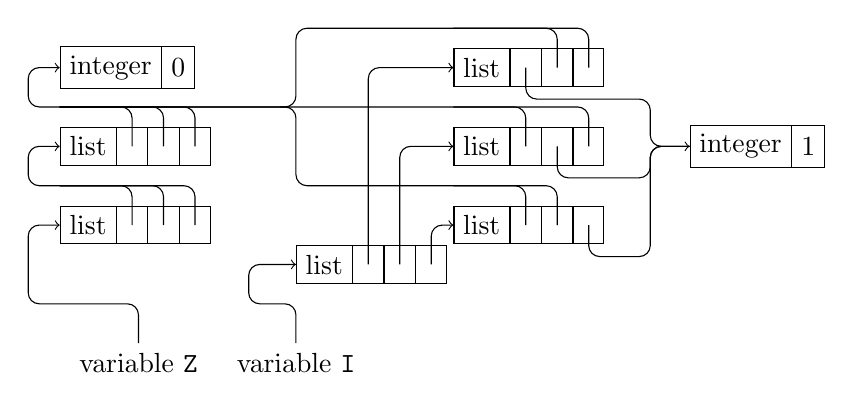
\begin{tikzpicture}[tclobj/.style={shape=rectangle split, 
        rectangle split parts=#1, rectangle split horizontal, draw, 
        anchor=west},tclobj/.default=2,
        pointer/.style={rounded corners=4pt}]
      \def\partmid#1{($(#1 south)!0.5!(#1 north)$)}
      \node[tclobj,name=0] at (0,2) {integer\nodepart{two}$0$};
      \node[tclobj=4,name=row] at (0,1) {list};
      \draw[pointer] \partmid{row.two}   |- (0,1.5);
      \draw[pointer] \partmid{row.three} |- (0,1.5);
      \draw[pointer,->] \partmid{row.four} |- (-0.4,1.5) |- (0.west);
      \node[tclobj=4,name=Z] at (0,0) {list};
      \draw[pointer]   \partmid{Z.two}   |- (0,0.5);
      \draw[pointer]   \partmid{Z.three} |- (0,0.5);
      \draw[pointer,->] \partmid{Z.four} |- (-0.4,0.5) |- (row.west);
      \node[tclobj,name=1] at (8,1) {integer\nodepart{two}$1$};
      \node[tclobj=4,name=I] at (3,-0.5) {list};
      \node[tclobj=4,name=I3] at (5,0) {list};
      \node[tclobj=4,name=I2] at (5,1) {list};
      \node[tclobj=4,name=I1] at (5,2) {list};
      \draw[pointer,->] \partmid{I.two}   |- (I1.west);
      \draw[pointer,->] \partmid{I.three} |- (I2.west);
      \draw[pointer,->] \partmid{I.four}  |- (I3.west);
      \draw[pointer,->] \partmid{I1.two} |- (7.5,1.6) |- (1.west);
      \draw[pointer] \partmid{I1.three} |- (5,2.5) -| (3,1.5) -- (0,1.5);
      \draw[pointer] \partmid{I1.four} |- (5,2.5);
      \draw[pointer] \partmid{I2.two}  |- (5,1.5);
      \draw[pointer] \partmid{I2.three} |- (7.5,0.6) |- (1.west);
      \draw[pointer] \partmid{I2.four} |- (2.8,1.5);
      \draw[pointer] \partmid{I3.two} |- (5,0.5);
      \draw[pointer] \partmid{I3.three} |- (5,0.5) -| (3,1.5) -- (0,1.5);
      \draw[pointer] \partmid{I3.four} |- (7.5,-0.4) |- (1.west);
      \draw[pointer,->] (1,-1.5) node[below] {variable \texttt{Z}} 
        |- (-0.4,-1) |- (Z.west);
      \draw[pointer,->] (3,-1.5) node[below] {variable \texttt{I}} 
        |- (2.4,-1) |- (I.west);
    \end{tikzpicture}
  \]
  \caption{Sharing of internal representations}
\end{figure}
However, if we were to make an 
identity matrix \verb|I| from \verb|Z| by changing the diagonal 
elements to $1$s through the commands
\begin{verbatim}
  set I $Z
  for {set k 0} {$k<$n} {incr k} {
     lset I $k $k 1 
  }
\end{verbatim}
(that \texttt{lset} does \(I_{k,k} := 1\)) then at each iteration of 
the loop the targetted row of \verb|I| will be copied before its $k$th 
element is changed to $1$, so the data structure storing the value of 
\verb|I| ends up with $n$ separate rows (as they need to be, since their 
values are distinct). 
There is still only one $0$ value, but now it is referenced $n^2$ 
times ($n-1$ times by each of the $n$ rows in \verb$I$, and another 
$n$ times by the only row in \verb$Z$, which of course remains 
unchanged), and the $1$ value is referenced $n$ times (once by each 
row of \verb$I$).

% The reason for explaining this in such detail is that in many other 
% programming languages, the default for such modifying operations is 
% rather to directly overwrite the original data, which would have 
% drastically different results: first the changes made to $I$ would be 
% seen also in $Z$, and if $Z$ was still cleverly reusing the same 
% row-of-zeroes $n$ times, then the result of the above could very well 
% be that $I$ (and $Z$) end up as the $n \times n$ matrices of all $1$s 
% (since each element in the only row has been separately overwritten 
% with that value). Correctly understanding the semantics of values 
% being immutable is crucial for some of the more intricate algorithms 
% in the completion utility; in particular the search-for-subnetwork 
% and list-all-overlaps operations rely heavily upon being able to 
% (cheaply) preserve the current state of a search by pushing the 
% values of the relevant variables onto a stack.


\subsubsection{Syntax and invariant descriptions}

Much of the practical syntax of \Tcl\ ends up being syntaxes of 
individual commands, and accordingly the official language 
documentation~\cite{tcl-lang-doc-8.6} is organised as one manpage per 
command. Some of these (e.g.~\verb|if|, \verb|try|) have rather complex 
clause-based syntaxes whereas others are more 
function-and-its-arguments (or verb-object-object-object-\dots\ if 
you want to go natural-language grammatical), but common to all is 
that the division into words is given. Accordingly, it seems appropriate 
to stress when some unit constitutes a word, so in what follows the 
familiar \meta{bar} notation for a metasyntactic variable is refined 
to \word{bar} when this unit is additionally to be exactly one word 
in a \Tcl\ sentence; the more generic \meta{bar} would still be used 
for part of a word or a sequence of (zero or more) words.

Pragmatically, it is also convenient to make use of certain notations 
from regular expressions---such as the \regopt, \regstar, and 
\regplus\ quantifiers---to express repetition variation in command 
syntaxes. For example
\begin{quote}
  \ttfamily
  list \word{element}\regstar\\
  incr \word{variable} \word{amount}\regopt
\end{quote}
means the \texttt{list} command takes zero or more \word{element}s, 
whereas the \texttt{incr} command takes a \word{variable} name and 
optionally also an \word{amount} by which to increment it. 
With parentheses to group pieces in such syntax expressions, the 
syntax of \verb|if| may be stated as
\begin{quote}
  \ttfamily\raggedright
  if \word{condition} then\regopt\ \word{script}
  $\bigl($elseif \word{condition} then\regopt\ 
  \word{script}$\bigr)\regstar$ $\bigl($else\regopt\ 
  \word{script}$\bigr)\regopt$
\end{quote}
showing not only that the final \texttt{else} clause is optional, but 
also that it may be preceeded by zero or more \texttt{elseif} 
clauses, and that the keywords \texttt{then} and \texttt{else} are 
optional.

These syntax conventions are in the completion utility sources 
applied not only to document individual commands, but also to 
document data structures, since the string representations of \Tcl\ 
lists are parsed into elements according to the same rules as \Tcl\ 
sentences are parsed into words; the main difference is that variable 
and command substitutions do not occur when parsing a list. Below it 
is the application of these conventions to lists and other data 
structures that is of more scientific interest, as data formats should 
be documented for posterity even if the programs that generated them 
may become obsolete.

To give an example, the string representation of a dictionary is
\begin{quote}
  \ttfamily
  $\bigl($\word{key} \word{value}$\bigr)\regstar$
\end{quote}
so the same as a list with an even number of elements, alternatingly 
having the roles of key and value. As a matter of general computer 
science, a \emph{dictionary} (associative array) is a sparse mapping 
of \word{key}s to \word{value}s. \Tcl\ implements dictionaries with a 
hashtable internal representation to achieve average $O(1)$ 
complexity for accessing individual elements; keys equality is string 
equality. 

Documentation may also need to state invariants and other propeties 
of the data structures considered, and for this it rather becomes 
appropriate to mix \Tcl\ code with ordinary mathematical formulae, 
when notation for some necessary operation exists only in one but 
not in the other. To signal what is what, \Tcl\ elements of such 
mixed formulae will appear in \texttt{typewriter} font and typically 
be delimited by command substitution brackets \texttt{[]}, whereas 
standard mathematical elements use normal formula fonts (e.g.~math 
italic). A trivial example is
\[
  \text{\ttfamily [lindex [list $a$ $b$ $c$] $1$]} = b
\]
where three values $a$, $b$, and $c$ are given to the \texttt{list} 
command to build a list with those three as elements. Then this list 
is passed to the \texttt{lindex} command that goes on to extract the 
element in position $1$ from this list; since \Tcl\ indexing is 
$0$-based, that will be the second element $b$. Finally at the top 
level of this mixed formula we assert mathematical equality $=$ of the 
value returned by that \texttt{lindex} to $b$. The standard 
mathematical formula language lacks good notation for this kind of 
construction and indexing operations---we rather prefer to give names 
to all elements we need to access---and programming languages 
conversely have little notation for stating claims, as programs are 
mainly about giving orders.



\section{The network datatype library}

The informal specification for a network is that is should be like a 
term (in the logic sense, i.e., a formalised expression), except that 
the underlying combinatorial structure should be that of a directed 
acyclic graph~(\smaller{DAG}) rather than a tree, because it needs to 
accomodate co-operations as well as ordinary operations. Formalising 
that does however require sorting out exactly what sense of `tree' we 
will generalise.

The tree structure of a term can be defined as the tree which as 
vertices has the subterms of the term and links two vertices with an 
edge if one is a maximal proper subterm of the other, but for our 
purposes it is more convenient to take as vertices the 
\emph{operations} (function symbols, including as nullary operations 
any named constants); this turns the tree into a kind of data-flow 
diagram (Figure~\ref{Fig:TermTrees&network}, middle). 
\begin{figure}
  \[
    \begin{tabular}{c@{\qquad}c@{\qquad}c}
      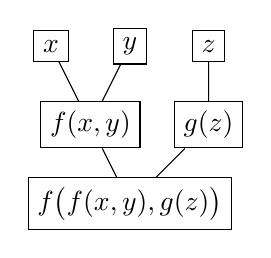
\begin{tikzpicture}
        \node[draw] (r1c1) at (0,2) {$x$};
        \node[draw] (r1c2) at (1,2) {$y$};
        \node[draw] (r1c3) at (2,2) {$z$};
        \node[draw] (r2c12) at (0.5,1) {$f(x,y)$};
        \node[draw] (r2c3) at (2,1) {$g(z)$};
        \node[draw] (r3c2) at (1,0) {$f\bigl( f(x,y), g(z) \bigr)$};
        \draw (r1c1) -- (r2c12) 
              (r1c2) -- (r2c12) 
              (r2c12) -- (r3c2)
              (r1c3) -- (r2c3) -- (r3c2);
      \end{tikzpicture}%
      &
      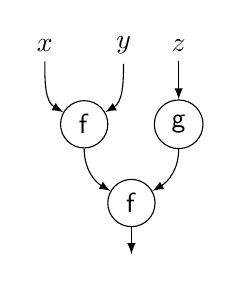
\begin{tikzpicture}[>=latex]
        \node (r1c1) at (0,2) {$x$};
        \node (r1c2) at (1,2) {$y$};
        \node (r1c3) at (1.7,2) {$z$};
        \node[draw,circle] (r2c12) at (0.5,1) {$\mathsf{f}$};
        \node[draw,circle] (r2c3) at (1.7,1) {$\mathsf{g}$};
        \node[draw,circle] (r3c2) at (1.1,0) {$\mathsf{f}$};
        \draw[->] (r1c1) to[out=-90,in=150] (r2c12);
        \draw[->] (r1c2) to[out=-90,in=30] (r2c12);
        \draw[->] (r2c12) to[out=-90,in=150] (r3c2);
        \draw[->] (r1c3) -- (r2c3);
        \draw[->] (r2c3) to[out=-90,in=30] (r3c2);
        \draw[->] (r3c2) -- ++(0,-0.65);
      \end{tikzpicture}%
      &
%       \begin{tikzpicture}
%         \node (r1c1) at (0,2) {$x$};
%         \node (r1c2) at (1,2) {$y$};
%         \node (r1c3) at (2,2) {$z$};
%         \node[draw,circle] (r2c12) at (0.5,1) {$\mathsf{f}$};
%         \node[draw,circle] (r2c3) at (2,1) {$\mathsf{\Delta}$};
%         \node[draw,circle] (r3c2) at (1,0) {$\mathsf{f}$};
%         \node[draw,circle] (r3c3) at (2.5,0) {$\mathsf{g}$};
%         \draw (r1c1) to[out=-90,in=150] (r2c12) 
%               (r1c2) to[out=-90,in=30] (r2c12) 
%               (r2c12) to[out=-90,in=135] (r3c2)
%               (r1c3) -- (r2c3) 
%               (r2c3) to[out=-135,in=45] (r3c2)
%               (r3c2) -- ++(0,-0.65)
%               (r2c3) to[out=-45,in=90] (r3c3)
%               (r3c3) -- ++(0,-0.65);
%       \end{tikzpicture}%
      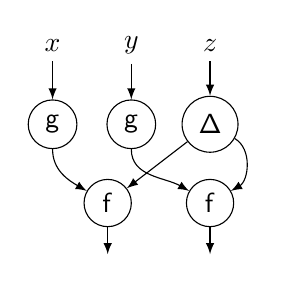
\begin{tikzpicture}[>=latex]
        \node (r1c1) at (0,2) {$x$};
        \node (r1c2) at (1,2) {$y$};
        \node (r1c3) at (2,2) {$z$};
        \node[draw,circle] (r2c1) at (0,1) {$\mathsf{g}$};
        \node[draw,circle] (r2c2) at (1,1) {$\mathsf{g}$};
        \node[draw,circle] (r2c3) at (2,1) {$\mathsf{\Delta}$};
        \node[draw,circle] (r3c2) at (0.7,0) {$\mathsf{f}$};
        \node[draw,circle] (r3c3) at (2,0) {$\mathsf{f}$};
        \draw[->] (r1c1) -- (r2c1);
        \draw[->] (r1c2) -- (r2c2);
        \draw[->] (r1c3) -- (r2c3);
        \draw[->] (r2c1) to[out=-90,in=150] (r3c2);
        \draw[->] (r2c2) to[out=-90,in=150] (r3c3);
        \draw[->] (r2c3) -- (r3c2);
        \draw[->] (r2c3) to[out=-30,in=30] (r3c3);
        \draw[->] (r3c2) -- ++(0,-0.65);
        \draw[->] (r3c3) -- ++(0,-0.65);
      \end{tikzpicture}%
      \\
      subexpressions tree& operations tree& 
      network
    \end{tabular}
  \]
  \caption{Term trees and a network}
  \label{Fig:TermTrees&network}
\end{figure}
The reason this structure for an ordinary term will be a rooted tree 
is that each operation syntactically produces exactly one result, but 
that is not the case with co-operations; paths taken by data within 
the expression may branch as well as join, creating a general 
\smaller{DAG} rather than a tree. The problem of how to even 
interpret such combinatorial objects as expressions is nontrivial, 
but turns out to have a natural solution~\cite[Sec.~5]{NR1}.

It is important to note that already an operations tree needs more 
structure than just the tree graph to encode a term. For one thing, 
there are the operation symbols \emph{decorating} the vertices, but 
more importantly the children of an operation are not interchangeable 
(unless that operation is commutative, but this is not a property 
that would be encoded into the syntax of a formula)---instead each 
incoming edge is attached to a separate \emph{port} of the vertex, 
and the set of available ports depend on the operation symbol; for 
example a binary operation has one `left operand' port and a 
separate `right operand' port. In a network the set of outgoing ports 
similarly depends on the operation symbol, so that for example a 
vertex for the coproduct $\mathsf{\Delta}$ has one incoming port but 
two outgoing ports. Finally networks are \emph{open graphs} in that 
they can have external edges signifying output (results) from a 
network and input (arguments) to it. In comparison to traditional 
terms the incoming external edges assume the role of free variables, 
which has interesting consequences for the rewrite theory: rewrite 
linearity becomes a syntactic requirement (although having 
co-operations allows for effectively reintroducing nonlinearity via 
explicit rules) and unification is no longer a primitive operation.


\subsection{Pure networks}
\label{Ssec:PureNetwork}

Mathematically, \cite{NR1}~defines a network as a tuple
\[
  G = (V,E,h,g,t,s,D)
\]
where \(\N \supset V \supseteq \{0,1\}\) and \(E \subset \N\) are the 
sets of vertices and edges of the underlying directed acyclic graph 
$(V,E,h,t)$ in which \(h,t\colon E \longrightarrow V\) are the 
functions mapping every edge $e$ to its head $h(e)$ and tail $t(e)$ 
respectively. To turn this into an open graph, the two mandatory 
vertices $0$ and $1$ are fixed as representing the output and input 
respectively sides of a network; an edge $e$ is outgoing external if 
it has \(h(e)=0\) and incoming external if it has \(t(e)=1\). 
Requiring that vertices and edges (or technically: the \emph{labels} 
of vertices and edges) are all natural numbers have certain 
set-theoretic advantages for defining isomorphism classes of 
networks, which are technically the objects that are being rewritten. 
The two functions \(g,s\colon E \longrightarrow \Z_{>0}\) map an edge 
(label) to the head and tail respectively \emph{index}, which 
identify the ports to which the edge is attached. Finally $D$ with a 
domain of $V \setminus \{0,1\}$ is the function mapping inner 
vertices to the operation symbols by which these are decorated. Such 
a symbol $x$ is given with an \emph{arity} $\alpha(x)$ and a 
\emph{coarity} $\omega(x)$ that are equal to the in-degree and 
out-degree respectively of any vertex decorated with~$x$. One also 
speaks about arity $\alpha(G)$ and coarity $\omega(G)$ of an entire 
network; these are the numbers of inputs and outputs to the network 
$G$ as a whole (thus technically the \emph{out}-degree of $1$ and 
\textit{in}-degree of $0$, respectively).

This mathematical concept is implemented in the network library as the 
datatype of \emph{pure networks}.
For ease of access, pure networks are implemented as heterogeneous 
nested lists, where some nesting levels act as records whereas others 
act as arrays. At the top level there is simply a pair
\begin{quote}
  \word{vertices} \word{edges}
\end{quote}
where \word{vertices} and \word{edges} are both lists indexed by 
vertex or edge respectively label; the sets $V$ and $E$ are implicit 
in the lengths $n$ and $m$ of these lists, since the vertex and edge 
labels are the indices of elements therein: \(V = \{0,\dotsc, n 
-\nobreak 1\}\) and \(E = \{0, \dotsc, m -\nobreak 1\}\). The element 
at any index $e$ in \word{edges} is a record-like list of the 
following four integers
\begin{quote}
  \word{$h(e)$} \word{$g(e)-1$} \word{$t(e)$} \word{$s(e)-1$}
\end{quote}
i.e., it specifies the head vertex label, head index, tail vertex 
label, and tail index; the only variation from the mathematical 
definition is that the indices are $0$-based.

This leaves only the decoration map $D$ to encode, but the 
\word{vertices} also duplicates the incidence information from 
$(h,g,t,s)$, to make traversing the network efficient. To that end, 
an element of \word{vertices} is a record-like list
\begin{quote}
  \word{decoration} \word{out-edges} \word{in-edges}
\end{quote}
where \word{decoration} is the value of $D$ at that vertex (or an 
empty string for the external vertices $0$ and $1$), \word{out-edges} 
is the list of labels of the outgoing edges in the order given by 
their tail-indices, and \word{in-edges} similarly is the list of 
labels of the incoming edges in the order given by their 
head-indices. For every network $G$ and every edge label $e$ of that 
network, it is an invariant that
\begin{multline*}
  \texttt{[lindex $G$ 0 [lindex $G$ 1 $e$ 0] 2 [lindex $G$ 1 $e$ 1]]}
  = \\ e =
  \texttt{[lindex $G$ 0 [lindex $G$ 1 $e$ 2] 1 [lindex $G$ 1 $e$ 3]]}
  \text{.}
\end{multline*}
A network
\begin{math}
  \begin{sdpgf}{0}{0}{60}{-124}{0.15pt}
    \m 41 -51 \C 20 20 -46 10 0 16 \S \m 19 -51 \C -20 20 46 10 0 16
    \S \m 30 -119 \L 0 41 \S \ov 14 -78 32 32 \S
  \end{sdpgf}
\end{math}
where the only operation vertex has a decoration `\texttt{m}' (for 
multiplication) can thus be encoded as the $69$~characters string
\begin{quote}
  \verb|{{{} {} 2} {{} {0 1} {}} {m 2 {1 0}}} |%
  \hfil\penalty151\hfilneg
  \verb|{{2 1 1 0} {2 0 1 1} {0 0 2 0}}|
\end{quote}
Though in some ways ``wasteful'' (for example using decimal digits to 
express numbers), this is actually quite compact in comparison to 
what it would take to realise the same graph structure with pointers 
on a contemporary architecture: a $64$-bit pointer is $8$ bytes, and 
with $3$ edges each containing $2$ pointers to vertices, times 
another $2$ because the vertices have to point back, that would be a 
minimum of \(8 \cdot 3 \cdot 2 \cdot 2 = 96\)~bytes for just tying 
the \smaller{DAG} together. Subsection~\ref{Ssec:Database} explains how 
outright compression is used to achieve further savings for long-term 
storage of networks.

% Because the \word{out-edges} of vertex $0$ and the \word{in-edges} of 
% vertex $1$ are always empty, an alternative encoding design could be 
% to combine the two external vertices into one, but doing so would 
% probably introduce 


\begin{topic}[Expressing networks] \label{Topic:Scanlines}
  One practical problem that faces a user of the network library is 
  how to construct any networks for it to operate on in the first 
  place, as writing down by hand a string representation such as the 
  above is not very convenient. The \texttt{network::pure::construct} 
  procedure provides a more practical interface where the user 
  provides a textual ``scanlist'' of the items in the network---lines 
  in order top (input side) to bottom (output side), and within each 
  line going left to right---that is easy to write down when looking 
  at a drawing of the network, and with some practice possible to 
  compose even without a drawn original. Inner vertex items are in the 
  scanlist expressed as their decorations; one needs to first declare how many 
  incoming and outgoing edges each vertex type has. Furthermore one 
  may write `\texttt{.}' for an edge merely passing through a 
  scanline, `\texttt{X}' for two edges crossing (or more generally 
  \texttt{\meta{$k$}X\meta{$l$}} for a crossing of $k$ edges going 
  down--right and $l$ edges going down--left), and a newline 
  (\verb|\n| or \verb|\r|) to mark the end of a scanline. This way, 
  the above 
  \begin{math}
    \begin{sdpgf}{0}{0}{60}{-124}{0.15pt}
      \m 41 -51 \C 20 20 -46 10 0 16 \S \m 19 -51 \C -20 20 46 10 0 16
      \S \m 30 -119 \L 0 41 \S \ov 14 -78 32 32 \S
    \end{sdpgf}
  \end{math}
  network can be written as `\verb|X \n m|' and the network on the 
  right in Figure~\ref{Fig:TermTrees&network} can be written 
  `\verb|g g Delta \n . X . \n f f|'.
\end{topic}

An alternative interface for entering networks into the program, 
which would probably be more appealing to the beginner, could be a 
graphical point-and-click approach; the actual programming is not 
very difficult. However even in a mainly graphical interface the 
scanlines seem to be a valuable abstraction to maintain, as they 
lessen the amount of graphical details that the user would have to 
provide.


\begin{topic}[Network isomorphism]
  Since the objects of algebraic interest are isomorphism classes of 
  networks, the library must provide for deciding network 
  isomorphism. It does so via the \texttt{network::pure::canonise} 
  command, which given any network returns a canonical representative 
  from the same isomorphism class; two networks are isomorphic if and 
  only if their respective canonical representatives are equal as 
  strings. Moreover the only way in which isomorphic networks may 
  differ is in how the individual vertices and edges are labelled, so 
  what the \texttt{canonise} operation concretely does is that it 
  generates a canonical labelling of the network.
  
  Canonical labelling of simple graphs is quite complicated due to 
  their flexible nature where vertices and edges have no identity 
  except as in relation to each other, but networks are far more rigid: 
  since edges attach to separate ports of a vertex, the identities of 
  all vertices in a component become fixed as soon as one fixes the 
  identity of one vertex. In addition the $0$ and $1$ vertices of a 
  network are already fixed, so in most networks that are encountered 
  there is already some way of identifying everything; what remains 
  is to turn that into a deterministic (not depending on labels in 
  the input) labelling scheme. The scheme 
  that is used is to do a breadth-first search through a graph 
  containing both vertices and edges of the network, each vertex 
  looking at incident edges in a deterministic order and likewise 
  each edge looking at its endpoints in a deterministic order. The 
  canonical labels are assigned sequentially in the order vertices 
  and edges are encountered by this search, and the search starts 
  with vertices $0$ and $1$ already enqueued. 
  
  Things get trickier for networks with components that are isolated 
  from both the output and the input; rewrite systems often have 
  rules that make these disappear, but during the intermediate steps 
  they must still be canonically labelled. This is done by first 
  computing a separate ``simplified'' canonical representation for 
  each component, sorting the components by the string representation 
  of this simplified representation, and finally assigning canonical 
  labels component by component; the exact ordering of the components 
  is irrelevant as long as it is deterministic, and equal components 
  simply appear in sequence.
  
  The simplified canonical representations are in turn obtained from 
  breadth-first searches of the individual components. Here we have 
  no canonical starting point for the search, so instead the search 
  is done multiple times with different vertices as starting point, 
  and whatever simplified representation happens to have the 
  lexicographically smallest string representation is picked as the 
  canonical one; since alternatives are considered only for the 
  starting point, the algorithm as a whole remains comfortably 
  polynomial. The 
  \texttt{network:\discretionary{}{}{}:pure:\discretionary{}{}{}:canonise} 
  command has a slight optimisation in that only vertices decorated by the 
  lexicographically smallest symbol found in a component are 
  considered as roots for the search in that component, but this can 
  at best improve the constant factor of the asymptotic complexity.
\end{topic}

Overall, canonical representations should probably not be expected to 
remain the same between different codebases; a programmer would be 
wise to treat any network as not canonical in the current process 
until it has been explicitly canonised. In particular, most 
library subroutines that produce networks will not bother to 
canonise them.

Case in point, the library provides a number of operations on 
networks that correspond to basic operations in the free \PROP---the 
elements of the free \PROP\ being isomorphism classes of networks, 
these network operations produce one representative from the 
equivalence class that is the result of applying the corresponding 
\PROP\ operation to the equivalence class(es) of the argument(s). 
In the \texttt{network::pure} namespace we find
\begin{ttdescription}
  \item[composition]
    Serial composition $\circ$ of one or more networks.
  \item[tensorprod]
    Parallel composition (tensor product) $\otimes$ of zero or more 
    networks.
  \item[permutation]
    Construct a permutation network, where all inputs are also 
    outputs.
  \item[left\_action]
    Permutate outputs of a network.
  \item[right\_action]
    Permutate inputs of a network.
  \item[substitute]
    Replace individual vertices of a network by other networks, 
    gadget style; this corresponds to applying a \PROP\ homomorphism 
    that one gets from the universal property of a free \PROP.
\end{ttdescription}
These are however only in rare cases immediately useful for 
rewriting. Instead rewriting is more easily expressed in terms of 
\emph{surgery} on networks, where some edges are cut, the detached 
pieces removed, and other pieces spliced into their place.

\begin{topic}[Regions in networks]
  A useful concept for describing surgical operations is that of a 
  \emph{region} in a network. This is by the library encoded as a list
  \begin{quote}
    \word{vertices} \word{outputs} \word{inputs}
  \end{quote}
  where \word{vertices} is a list of vertex labels and the other two 
  lists of (primarily) edge labels. Regions defining the ambiguity 
  processed are recorded in the database by the completion utility, 
  which is why their encoding should be documented.
  The concept in~\cite{NR1} that corresponds to regions is that of 
  \emph{strong embedding} of a network into another.
  
  If for intuition viewing a network as a topological space, then a 
  region is a (finitely presented) open subset thereof; in 
  particular, if a vertex is in the region then also (at least parts 
  of) the edges incident with that vertex must be included. Outputs 
  and inputs of the network must however be listed explicitly, since 
  the subnetwork selected by the region always has its outputs and 
  inputs in some specific order. An edge not occurring in the 
  \word{outputs} or \word{inputs} must either be wholly in the region 
  and thus have both its endpoints in the \word{vertices}, or wholly 
  outside the region and thus have neither of its endpoints in the 
  \word{vertices}.
  
  A complication that arises is that edges sometimes are decomposed 
  into more than two pieces by the region boundary---a single edge 
  may appear arbitrarily many times in the \word{outputs} and 
  \word{inputs}, if the intermediate pieces in the selected 
  subnetwork count as edges going directly from input side to output 
  side. To keep track of which part connects to what, the elements of 
  \word{outputs} and \word{inputs} are in fact integers $e+mi$ where 
  \(e \in E\) is the edge label proper, \(m = \lvert E\rvert\) is the 
  total number of edges, and \(i \in \mathbb{N}\) is an index to 
  distinguish the separate pieces the region has of edge $e$; lower 
  index values are closer to the tail of the edge. 
  Figure~\ref{Fig:Region} shows an example of a network with a 
  region, that also exhibits a multipart edge.
\end{topic}

\begin{figure}
  Given that \texttt{m} has arity $2$ and coarity $1$, \texttt{Delta} 
  has arity $1$ and coarity $2$, and finally \texttt{S} has arity and 
  coarity both $1$, the scanlist
  \begin{quote}
    \verb|Delta . \n . Delta S \n m m|
  \end{quote}
  constructs a network $G$ with encoding
  \begin{quote}
    \ttfamily\makebraceother
    {{{} {} {7 8}} {{} {2 3} {}} {Delta {0 1} 2} {Delta {4 5} 1} 
    {S 6 3} {m 7 {0 4}} {m 8 {5 6}}} 
    {{5 0 2 0} {3 0 2 1} {2 0 1 0} {4 0 1 1} {5 1 3 0} {6 0 3 1} 
    {6 1 4 0} {0 0 5 0} {0 1 6 0}}
    \makebracegroups
  \end{quote}
  In particular it has \(V = \{0,1,2,3,4,5,6\}\) and \(E = 
  \{0,1,2,3,4,5,6,7,8\}\); the inner vertices $2$ through $6$ are 
  exactly in the scanlist order. A region in this network is
  \begin{quote}
    \ttfamily\makebraceother
    {2 3 6} {0 9 4 8} {2 9 6}
    \makebracegroups
  \end{quote}
  which is shown with thick lines in subfigure~(a) below. Note how 
  edge~$0$ (the leftmost one) has two segments in the region (and two 
  outside it).
  \[
    \text{(a):}\quad
    \left[ \begin{sdpgf}{0}{0}{150}{-268}{0.2pt}
      \m 90 -263 \C 0 7 4 7 4 6 \S \m 60 -26 \L 0 21 \S \m 120 -118 \C 0 16
      -15 14 0 16 \L 0 20 \C 0 16 -15 15 0 16 \S \m 122 -174 \C 0 8 -2 8 0
      8 \S \m 60 -263 \C 0 14 -15 13 0 14 \S \m 15 -134 \L 0 10 \C 0 5 1 5
      2 4 \S \m 34 -195 \C -10 10 -6 14 -2 13 \S \m 56 -195 \C 8 8 -6 8 -5
      9 \S \begin{pgfscope} \pgfsetlinewidth{3\pgflinewidth} \m 98 -243 \C
      3 7 4 7 0 7 \S \m 53 -170 \C -6 9 -6 8 8 8 \S \m 18 -110 \C 6 14 14
      12 11 11 \S \m 94 -195 \C -13 13 3 24 -13 13 \S \m 60 -118 \C 0 15 25
      16 -14 14 \S \m 16 -158 \C -1 5 0 5 0 4 \L 0 10 \S \m 116 -195 \C 6 6
      1 7 -1 8 \S \m 60 -46 \L 0 20 \S \end{pgfscope} \ov 44 -78 32 32 \S
      \ov 44 -150 32 32 \S \re 104 -150 32 32 \S \ov 29 -222 32 32 \S \ov
      89 -222 32 32 \S
    \end{sdpgf} \right]
    \qquad
    \text{(b):}\quad
    \left[ \begin{sdpgf}{0}{0}{150}{-268}{0.2pt}
      \m 109 -195 \C -13 13 18 24 -13 13 \S \m 30 -263 \C 0 16 -15 15 0 16
      \L 0 20 \L 0 52 \L 0 20 \C 0 18 6 20 13 13 \S \m 120 -263 \L 0 41 \S
      \m 90 -118 \C 0 19 -20 12 -14 14 \S \m 131 -195 \C 13 13 -9 21 0 17
      \L 0 20 \C 0 18 -15 16 0 18 \L 0 20 \C 0 16 -15 15 0 16 \S \m 45 -46
      \L 0 41 \S \m 60 -263 \C 0 16 -15 15 0 16 \L 0 20 \L 0 52 \L 0 20 \C
      0 24 45 4 0 24 \L 0 20 \C 0 16 -15 15 0 16 \S \m 90 -263 \C 0 16 -15
      15 0 16 \L 0 20 \C 0 17 -9 21 13 13 \S \ov 29 -78 32 32 \S \ov 74
      -150 32 32 \S \ov 104 -222 32 32 \S
    \end{sdpgf} \right]
    \qquad
    \text{(c):}\quad
    \left[ \begin{sdpgf}{0}{0}{210}{-174}{0.2pt}
      \m 180 -169 \L 0 41 \S \m 30 -169 \L 0 41 \S \m 19 -101 \C -69 69 185
      -11 0 38 \S \m 60 -169 \C 0 23 45 1 0 23 \L 0 20 \C 0 47 90 3 0 47 \S
      \m 41 -101 \C 37 37 87 5 0 54 \S \m 120 -169 \C 0 23 -45 1 0 23 \L 0
      20 \C 0 39 -60 19 0 39 \S \m 150 -169 \C 0 16 -15 15 0 16 \L 0 20 \C
      0 33 -30 31 0 33 \S \m 180 -96 \C 0 59 -135 -27 0 59 \S \re 164 -128
      32 32 \S \ov 14 -128 32 32 \S
    \end{sdpgf} \right]
  \]
  Subfigure~(b) is the selected subnetwork uncovered, showing also the 
  relative order between its inputs and outputs; the $9$ in the above 
  region is the second (index $1$) part of edge $0$, which is mostly 
  parallel to the first part of the same edge. 
  Subfigure~(c) is instead what remains of $G$ when the selected region 
  has been detached; inner inputs and outputs (those that connected 
  to the detached region) appear to the right of the original inputs 
  and outputs from~(a).
  
  \caption{Region in a network}
  \label{Fig:Region}
\end{figure}

The outright \texttt{replace}ment of a region in one network $G$ by a 
different network $H$ is both in the library and in~\cite{NR1} 
decomposed into separate operations of first \texttt{detach}ing the 
part of $G$ which was inside the region and then joining the part $K$ 
which remains up with the new piece $H$ using an \texttt{annex}ation 
operation $\rtimes$ to form a new network $K \rtimes H$ where all 
inputs of $H$ are joined to the last few outputs of $K$ and all 
outputs of $H$ are joined to the last few inputs of $K$; in the 
``$\rtimes H$'' part, edges are going 
$\rlap{$\nwarrow$}{\nearrow\mkern-4mu\downarrow\mkern-2mu}$. This 
last step in principle carries the risk of creating directed cycles 
in the result, but this risk is carefully managed; 
\cite[Sec.~7.1]{NR1} uses boolean matrices to keep track of exactly 
when such join operations are well-defined, and in the network 
library the concept of \emph{network with feedback} (next subsection) 
serves the same purpose. In particular, the operations that compute 
regions typically take networks with feedback as operands.

It should be observed that replacement of regions within a network is 
a \emph{more general} operation than rewriting by means of double 
pushouts. The reason for this is that the double pushout formalism 
produces left and right hand sides of a rewrite step as images of a 
common pattern network where a single vertex is mapped to the left 
and right hand sides of a rewrite rule, but regions are more general 
than what can be the image of a single vertex; an output of a region 
can connect back to an input of that region, whereas an output of a 
single vertex connecting back to an input of that vertex is 
immediately an acyclicity violation. Regions are said to be 
\emph{convex} if there is no directed path which leaves the region 
and then returns to it; any region obtained as the image of a single 
vertex will be convex, and double pushout rewriting is thus 
restricted to making convex replacements. It turns out completion 
frequently derives nonconvex rewrite rules, even if starting from a 
purely convex set of axioms.

\begin{topic}[Structural decomposition of networks] \label{Topic:NwDecompose}
  When networks are constructed through a sequence of replacements, 
  there is an obvious risk that any governing principle for their 
  structure---such as being produced through a sequence of serial and 
  parallel compositions---is destroyed; therefore it becomes 
  interesting to take a general network and seek a comprehensible 
  decomposition of it. Unfortunately this seems to be a difficult 
  problem, with no obvious solution. The network library contains a 
  number of procedures attacking this decomposition problem, but most 
  are dead code used for nothing. What exceptions there are 
  (Topics~\ref{Topic:LevelDecompose} and~\ref{Topic:LevelOrder}) 
  participate in the generation of graphical layouts for networks 
  (Topic~\ref{Topic:Layout}), and that is a major topic of its own.
\end{topic}


\begin{topic}[Monomial ordering of networks]
  Completion requires that the objects being rewritten can be 
  compared, so that derived equalities can be oriented into rewrite 
  rules. Similarly to Topic~\ref{Topic:NwDecompose}, the network 
  library contains a body of procedures written as experiments in 
  developing a useful ordering, but here the story has a happier 
  ending in that a good solution was eventually discovered, even if 
  it ended up not actually needing any of the code here.
  
  The theory for ordering networks is explained 
  in~\cite[Sec.~3]{NR1}: first construct any sufficiently fine 
  ordered \PROP\ $\mathcal{P}$---a good choice is the biaffine \PROP\ 
  over any partially ordered cancellative semiring---then use the 
  universal property of the free \PROP\ to pull this order back to 
  the networks. Practically one evaluates the networks one wishes to 
  compare in the \PROP\ $\mathcal{P}$, with some choice of value for 
  each element in one's signature, and then compares the values of the 
  networks as a whole. A suggested interface for implementations of 
  \PROPs~(see \texttt{props.dtx}) contains a \texttt{fuse} operation 
  that is straightforward to use to that end.
  
  As a matter of development history, this conceptually neat 
  construction evolved from the idea of making lexicographic 
  comparisons along all possible paths through the networks being 
  compared. An ordering that worked for orienting the axioms of a 
  bialgebra could be defined in that way, but for compatibility with 
  composition one needed to first make sure that the networks 
  being compared had the same number of paths for each combination of 
  input and output; this is similar to how in word rewriting one 
  needs to first compare by word length before one can make a 
  lexicographic comparison. However in the bialgebra case it was then 
  realised that already the path-counting stage (if slightly tweaked) 
  would suffice for oriented all rules as desired~\cite{LH:WST,NR2}; 
  the biaffine \PROP\ can be interpreted as precisely counting paths.
\end{topic}


\begin{topic}[Level decomposition of networks] 
  \label{Topic:LevelDecompose}
  A more modest goal compared to that of 
  Topic~\ref{Topic:NwDecompose} is to make a serial decomposition of 
  a network $b$ as \(b_1 \circ \dotsb \circ b_l\) where each $b_i$ 
  only employs $\otimes$ and permutations. In~\cite[Sec.~4--5]{NR1} 
  this was done to the end of proving that networks indeed may be 
  interpreted as expressions for arbitrary \PROPs, by putting every 
  vertex in a level of its own, but that is often too drawn out 
  to be comprehensible. Instead it is useful to have a decomposition 
  into a minimal number of levels.
  
  The vertical\slash serial aspect of a level decomposition boils down 
  to what levels the vertices should be placed in, for which problem 
  there again exists a number of implementations in the library. The 
  current production procedure 
  \texttt{network:\discretionary{}{}{}:pure:}\discretionary{}{}{}%
  \verb|:vertex_levels4| conceptually treats the whole situation as a 
  linear programme with the vertical vertex positions as the 
  variables, inequalities expressing that every edge has to have 
  length at least $1$, and an objective of minimising the sum of all 
  edge lengths. In principle this linear programme is then solved 
  using the simplex algorithm (with infinitesimal pertubations to 
  avoid degenerate corners of the polytope), but in practice the 
  state of the algorithm boils down to keeping track of the edges for 
  a spanning tree in the network, since every edge corresponds to an 
  inequality and the set of tight inequalities are what determines 
  the current feasible point. In particular there is never a need to 
  solve a general linear equation system.
\end{topic}

The effect is similar to decomposing a network into scanlines as per 
Topic~\ref{Topic:Scanlines}, but different in that it allows for 
arbitrary permutations \emph{between} levels whereas the scanlines 
presentation only does permutations \emph{within} levels. Doing 
permutations between levels can sometimes lead to messy situations; 
in particular having several edges go many positions sideways can 
lead to them touching and making it hard to tell which is which. 
The network in Figure~\ref{Fig:Region}c has had its layout tweaked by 
(among other things) increasing the distance between the input level 
and the level below, so that the edges are distinct.


\begin{topic}[Order within network levels] \label{Topic:LevelOrder}
  Having assigned every vertex to a specific level, what remains for 
  producing a full layout is to somehow order the items within each 
  level. This is again a difficult problem with no obvious solution, 
  and naive algorithms such as trying all possibilities end up with 
  superexponential complexity. Moreover even the choice of an 
  appropriate objective function for comparing different orders is 
  not entirely trivial; several seemingly good ideas have turned out 
  to produce aesthetically unpleasing results. Thus the library again 
  contains a number of procedures to this end that have been found 
  wanting and are not used.
  
  The procedure \verb|network::pure::ordered_graded_components| 
  currently used in production works by having each level suggest 
  hints on how items should be ordered in adjacent levels, compiling 
  the hints received into a partial order, and then suggest new hints 
  based on relations exhibited by that partial order; repeat until 
  propagation dies down, make an arbitrary choice and repeat again 
  until all level orders are total. The initial suggestions come 
  primarily from the orders of indicent edges at each vertex, e.g.~a 
  vertex with two inputs would suggest to the level above that the 
  item connected to the first input is placed to the left of the item 
  connected to the second input. Conflicts between suggestions are 
  resolved simply by arbitrarily picking one of them, and never 
  backtracking once a choice has been made. This works fairly well 
  when there indeed is close to a consensus on what should go left 
  and what should go right---with a slight reservation for the fact 
  that it has a tendency to make large jumps in order at the boundary 
  between two ``zones of influence'' (see 
  Figure~\ref{Fig:ZonesOfInfluence}) rather than many small 
  jumps to gradually switch between two conflicting opinions---but 
  appears to produce less aesthetically pleasing results when there 
  is much conflict; however it has not been systematically examined 
  to what extent there even exists more pleasing layouts in those 
  cases.
  
  \begin{figure}
    \[
      \text{(a):}\quad
      \vcenter{
        \hbox{\verb|Delta \n|}
        \hbox{\verb|X \n|}
        \hbox{\verb|Delta Delta \n|}
        \hbox{\verb|m m \n|}
        \hbox{\verb|m|}
      }
      \qquad
      \text{(b):}\quad
      \left[ \begin{sdpgf}{0}{0}{120}{-340}{0.2pt}
        \m 71 -267 \C 12 12 7 17 0 16 \S \m 41 -195 \C 14 14 0 22 -14
        14 \S \m 90 -118 \C 0 16 -68 2 27 27 \S \m 60 -335 \L 0 41 \S
        \m 79 -195 \C -14 14 0 22 14 14 \S \m 30 -118 \C 0 16 68 2 -27
        27 \S \m 101 -195 \C 14 14 0 22 -14 14 \S \m 60 -46 \L 0 41 \S
        \m 49 -267 \C -12 12 -7 17 0 16 \S \m 19 -195 \C -14 14 0 22
        14 14 \S \ov 44 -78 32 32 \S \ov 14 -150 32 32 \S \ov 74 -150
        32 32 \S \ov 14 -222 32 32 \S \ov 74 -222 32 32 \S \ov 44 -294
        32 32 \S
      \end{sdpgf} \right]
      \qquad
      \text{(c):}\quad
      \left[ \begin{sdpgf}{0}{0}{120}{-340}{0.2pt}
        \m 71 -267 \C 12 12 7 17 0 16 \S \m 41 -195 \C 20 20 68 2 -28
        28 \S \m 30 -118 \C 0 16 7 17 12 12 \S \m 60 -335 \L 0 41 \S
        \m 79 -195 \C -20 20 -68 2 28 28 \S \m 90 -118 \C 0 16 -7 17
        -12 12 \S \m 101 -195 \C 28 28 -68 2 -20 20 \S \m 60 -46 \L 0
        41 \S \m 49 -267 \C -12 12 -7 17 0 16 \S \m 19 -195 \C -28 28
        68 2 20 20 \S \ov 44 -78 32 32 \S \ov 74 -150 32 32 \S \ov 14
        -150 32 32 \S \ov 14 -222 32 32 \S \ov 74 -222 32 32 \S \ov 44
        -294 32 32 \S
      \end{sdpgf} \right]
    \]
    Subfigure~(a) is the scanlist used to describe a network, divided 
    into lines to clarify the structure. Subfigure~(b) is the network 
    layout one might expect from that scanlist, but due to the zones 
    of influence phenomenon, the layout produced from the pure network 
    is rather that of Subfigure~(c): on the first round, the top and 
    bottom vertices get to suggest how their neighbours should be 
    ordered, and since there at that point are no suggestions to the 
    contrary, these suggestions stick.
    \caption{The ``zones of influence'' effect}
    \label{Fig:ZonesOfInfluence}
  \end{figure}
  
  Aesthetically superior heuristics for network layouts would be a 
  valuable addition, but the current ones do have the virtue of being 
  quick enough to execute and good enough so far.
\end{topic}



\subsection{Networks with feedback}
\label{Ssec:WithFeedback}

A \emph{network with feedback} is defined as a pair
\begin{quote}
  \word{network} \word{feedback-list}
\end{quote}
where in turn a \word{feedback-list} is a list (order irrelevant, so 
effectively a set) of pairs $(i,j)$ encoding the sentiment that the 
output with index $i$ of the \word{network} may be fed back into the 
input with index $j$ of that same network. When looking for redexes 
at which to apply a rewrite rule to a network, one must take into 
account not only the \word{network} that constitutes the left hand 
side of the rule, but also whether the region into which this network 
gets embedded satisfies the dependency constraints under which that 
rule was derived, i.e., would it be possible to replace this single 
rule step by a sequence of more elementary rewrite steps while still 
preserving acyclicity of all intermediate networks? Those are exactly 
the constraints expressed by the \word{feedback-list}: one may not 
have a directed path from output $i$ returning back to input $j$ 
unless the pair $(i,j)$ is in the \word{feedback-list}.

A related concept is that of the \emph{transferrence} of a network $G$, 
which is the boolean $\omega(G) \times \alpha(G)$ matrix 
$\operatorname{Trf}(G)$ that has a $1$ in position $(i,j)$ if and 
only if there is a directed path in $G$ from input $j$ to output $i$. 
In~\cite[Sec.~7--8]{NR1} it is proved that $\operatorname{Trf}$ may also 
be interpreted as a \PROP\ homomorphism from the free \PROP\ to the 
\PROP\ $\mathbb{B}^{\bullet\times\bullet}$ of boolean matrices. Taking 
into account that the standard order of boolean matrices (the partial 
order doing elementwise comparisons) is compatible with this \PROP\ 
structure, we even get that the free \PROP\ is equipped with a 
$\mathbb{B}^{\bullet\times\bullet}$-filtration $\{ \mathcal{F}_q 
\}_{q \in \mathbb{B}^{\bullet\times\bullet}}$ called the dependency 
filtration, defined by the condition that \([G] \in \mathcal{F}_q\) 
iff \(\operatorname{Trf}(G) \leqslant q\). The \emph{formal feedback} 
structure~\cite[Sec.~9]{NR1} on the free \PROP\ is that a variety of 
connect-output-back-to-input operations ($\rtimes$, $\Join$, and 
$\uparrow$) can be defined as \emph{total} (not just partial) 
operations on appropriate components in this dependency filtration, 
and also that their codomains are again found in this filtration.

\begin{topic}[Mathematical interpretation of feedbacks]
  \label{Topic:Feedbacks}
  Within the completion utility, the feedbacks primarily matter for 
  operations that are looking for matches of (part of) one network 
  with feedback to (part of) another network with feedback, by going 
  through a search tree of ways to match the underlying pure networks. 
  If during this search a path arises from an output to an input which 
  is not listed among the feedbacks of this network, then the 
  feedback constraints have been violated and the search backtracks. 
  While the completion utility was being developed, this was pretty 
  much the extent to which the feedbacks had any interpretation.
  
  The theoretical foundations in~\cite[Sec.~10]{NR1} are that the 
  networks being rewritten live in a particular component of the 
  dependency filtration $\{\mathcal{F}_q\}_{q \in 
  \mathbb{B}^{\bullet\times\bullet}}\), and that rewrite rules do the 
  same. Since the operation of feeding output $i$ back to input $j$ is 
  well-defined for \(\mu \in \mathcal{F}_q\) if and only if 
  \(q_{i,j}=0\), the interpretation of the \word{feedback-list} 
  became that this is a sparse encoding of this transferrence type 
  matrix $q$: all elements are $1$ except those whose positions 
  $(i,j)$ are given. Some later additions to the completion utility 
  explicitly make this interpretation when exporting\slash displaying 
  rewrite rules. It was however already in~\cite[Ex.~10.28]{NR1} 
  observed that this model had certain problems, and in~\cite{LH:IWC} 
  it was suggested that some further refinement might be needed.
  
  The present~(2021) understanding is rather that the 
  \word{feedback-list}s have the right amount of detail, but that 
  the original theoretical understanding of them is slightly off. 
  Rather than a pair $(j,i)$ signalling that element $(i,j)$ of an 
  $\omega(G) \times \alpha(G)$ boolean matrix $q$ is $0$, they signal 
  that element $(j,i)$ of an $\alpha(G) \times \omega(G)$ boolean 
  matrix $p$ is $1$, where $p$ keeps track of how the context is 
  allowed to connect things; rather than the constraint on 
  $\operatorname{Trf}(G)$ being \(\operatorname{Trf}(G) \leqslant 
  q\), it should be that $p \operatorname{Trf}(G)$ (a product of two 
  boolean matrices) is nilpotent. For \word{feedback-list}s with only 
  one element these two interpretations are equivalent, but when there 
  are more feedbacks the $p$ interpretation becomes more flexible.
\end{topic}


\begin{topic}[Finding subnetwork instances]
  In order to do rewriting, it is necessary to check if one network 
  (the rewrite rule left hand side) appears as a subnetwork of 
  another network (that being rewritten), and if so in what region. 
  The network library provides this functionality through the 
  \texttt{instances} procedure in the \texttt{network::wfb} (With 
  FeedBack) namespace. It works by searching through a tree of 
  candidate ways of identifying vertices and edges of the subnetwork 
  $H$ with the supernetwork $G$, offering to halt the search when a 
  certain number of matches (typically $1$ or $\infty$) has been 
  found.
  
  The search tree is typically quite shallow, since identifying one 
  vertex $v$ of $H$ with a vertex of $G$ will determine how the 
  entire component of $v$ is embedded into $G$ (or reveal that $v$ 
  would have to be embedded somewhere else). Subnetworks $H$ with 
  multiple components may however require several choices before an 
  embedding is fixed, and $H$ edges from input to output do in this 
  case count as separate components, which contributes to the code 
  complexity: there are two kinds of components to embed. Immutable 
  value semantics do however make it trivial to cache a copy of any 
  pre-choice state as something to return to after backtracking.
\end{topic}


\begin{topic}[Enumerating ambiguities]
  In order to do completion, it is necessary to enumerate all 
  (critical) ambiguities---minimal networks that can be reduced in 
  two different ways---and traditionally this is done by picking two 
  rewrite rules and listing all the ways in which their left hand 
  sides may be overlapped. The \texttt{ambiguities} procedure in the 
  \texttt{network::wfb} namespace does precisely this: given two 
  networks with feedback $H_1$ and $H_2$ it returns a list of 
  networks with feedback $G$ such that both $H_1$ and $H_2$ appear as 
  subnetworks of $G$, and also the regions where they do this. In the 
  terminology of~\cite{NR1}, the list returned covers all 
  \emph{decisive} ambiguities, which are exactly the ones that it 
  by the diamond lemma~\cite[Th.~10.24]{NR1} suffices to check.
  
  The algorithm used in the \texttt{ambiguities} procedure resembles 
  that of the \texttt{instances} procedure in that it explores a 
  search tree of all possibilities for how to identify vertices and 
  edges of the two networks, but here there is always also the 
  possibility that something in one network is not identified with 
  something in the other, which increases the tree valency a bit. It 
  is also not the case that components gets fixed by only one choice 
  each, because there is with networks no requirement that the 
  intersection of $H_1$ and $H_2$ (as embedded into $G$) is 
  connected; whenever there is a way of overlapping them in two 
  places, there will also be two more ambiguities in which $H_1$ and 
  $H_2$ overlap in just one of these places (see 
  Figure~\ref{Fig:OverlapChoices}). This is different from 
  the situation for trees\slash terms, which have the property that 
  the common part in an overlap of two trees is itself a tree and 
  thus connected.
  
  \begin{figure}
    \[
      \begin{array}{c@{\quad}c@{\qquad} c@{\quad}c@{\quad}c}
      \left[ \begin{sdpgf}{0}{0}{120}{-268}{0.2pt}
        \m 56 -195 \C 13 13 6 20 0 18 \L 0 20 \C 0 20 30 12 0 20 \L 0
        20 \C 0 16 -15 15 0 16 \S \m 19 -123 \C -13 13 9 21 0 17 \L 0
        20 \C 0 16 15 15 0 16 \S \m 34 -195 \C -11 11 7 19 0 15 \S \m
        41 -123 \C 13 13 -18 24 13 13 \S \m 45 -263 \L 0 41 \S \m 75
        -263 \C 0 16 15 15 0 16 \L 0 20 \C 0 18 15 16 0 18 \L 0 20 \C
        0 20 -19 16 -15 15 \S \m 60 -46 \L 0 41 \S \ov 44 -78 32 32 \S
        \ov 14 -150 32 32 \S \ov 29 -222 32 32 \S
      \end{sdpgf} \right]
      &
      \left[ \begin{sdpgf}{0}{0}{120}{-268}{0.2pt}
        \m 86 -195 \C 11 11 -7 19 0 15 \S \m 64 -195 \C -13 13 -6 20 0
        18 \L 0 20 \C 0 18 -15 16 0 18 \L 0 20 \C 0 16 15 15 0 16 \S
        \m 75 -263 \L 0 41 \S \m 45 -263 \C 0 16 -15 15 0 16 \L 0 20
        \C 0 18 -15 16 0 18 \L 0 20 \C 0 24 32 10 17 17 \S \m 90 -118
        \C 0 15 7 19 -11 11 \S \m 75 -46 \L 0 41 \S \ov 59 -78 32 32
        \S \re 74 -150 32 32 \S \ov 59 -222 32 32 \S
      \end{sdpgf} \right]
      &
      \left[ \begin{sdpgf}{0}{0}{180}{-268}{0.2pt}
        \m 75 -263 \C 0 14 -15 13 0 14 \S \m 105 -46 \L 0 41 \S \m 19
        -123 \C -15 15 26 19 0 17 \L 0 20 \C 0 16 15 15 0 16 \S \m 105
        -263 \C 0 14 15 13 0 14 \S \m 109 -195 \C -13 13 9 21 0 17 \L
        0 20 \C 0 24 45 4 0 24 \L 0 20 \C 0 16 -15 15 0 16 \S \m 71
        -195 \C 13 13 -9 21 0 17 \L 0 20 \C 0 18 -15 16 0 18 \L 0 20
        \C 0 16 15 15 0 16 \S \m 49 -195 \C -12 12 -7 17 0 16 \S \m 41
        -123 \C 17 17 19 16 17 17 \S \m 131 -195 \C 12 12 7 17 0 16 \S
        \m 150 -118 \C 0 19 -20 12 -14 14 \S \ov 89 -78 32 32 \S \ov
        14 -150 32 32 \S \re 134 -150 32 32 \S \ov 44 -222 32 32 \S
        \ov 104 -222 32 32 \S
      \end{sdpgf} \right]
      &
      \left[ \begin{sdpgf}{0}{0}{120}{-268}{0.2pt}
        \m 49 -195 \C -12 12 -7 17 0 16 \S \m 19 -123 \C -15 15 26 19
        0 17 \L 0 20 \C 0 16 15 15 0 16 \S \m 71 -195 \C 12 12 7 17 0
        16 \S \m 41 -123 \C 13 13 -3 24 13 13 \S \m 60 -263 \L 0 41 \S
        \m 90 -118 \C 0 15 7 19 -11 11 \S \m 75 -46 \L 0 41 \S \ov 59
        -78 32 32 \S \ov 14 -150 32 32 \S \re 74 -150 32 32 \S \ov 44
        -222 32 32 \S
      \end{sdpgf} \right]
      &
      \left[ \begin{sdpgf}{0}{0}{180}{-268}{0.2pt}
        \m 101 -195 \C 16 16 33 6 0 23 \S \m 120 -263 \C 0 16 15 15 0
        16 \L 0 20 \C 0 20 -30 12 0 20 \L 0 20 \C 0 18 6 20 13 13 \S
        \m 19 -123 \C -15 15 26 19 0 17 \L 0 20 \C 0 19 30 9 0 19 \S
        \m 90 -263 \L 0 41 \S \m 150 -118 \C 0 15 7 19 -11 11 \S \m 41
        -123 \C 13 13 -3 24 13 13 \S \m 135 -46 \C 0 14 -15 13 0 14 \S
        \m 60 -263 \C 0 16 -15 15 0 16 \L 0 20 \C 0 20 30 12 0 20 \L 0
        20 \C 0 17 26 19 -15 15 \S \m 79 -195 \C -16 16 -33 6 0 23 \S
        \m 75 -46 \C 0 14 15 13 0 14 \S \ov 59 -78 32 32 \S \ov 119
        -78 32 32 \S \ov 14 -150 32 32 \S \re 134 -150 32 32 \S \ov 74
        -222 32 32 \S
      \end{sdpgf} \right]
      \\
      H_1 & H_2 & G_1 & G_2 & G_3
      \end{array}
    \]
    Looking for ways of overlapping $H_1$ and $H_2$, all of $G_1$, 
    $G_2$, and $G_3$ are valid possibilities; there are separate 
    choices of whether to overlap the top vertices and whether to 
    overlap the bottom vertices. The $G_2$ overlap does however 
    require that $H_1$ and $H_2$ allow for feedbacks.
    \caption{Networks and overlaps}
    \label{Fig:OverlapChoices}
  \end{figure}
  
  Concretely the procedure begins with $H_1$ as $G$, then working its 
  way through the vertices of $H_2$ while choosing which if any $G$ 
  vertex with which to identify it. If an edge indicent with an 
  identified vertex is inner in both $H_1$ and $H_2$ then the other 
  endpoint of this edge is also enqueued for identification, whereas 
  if the edge is inner in $H_2$ but not so in $H_1$ then proceeding 
  requires making a choice: is the other endpoint a vertex in $H_1$ 
  (and if so which one) or not? The general story is that edges that 
  are inner in $H_1$ or $H_2$ will be mapped to inner edges of $G$, 
  but inputs and outputs of $H_1$ or $H_2$ may also be mapped to 
  inner edges of $G$, if feedbacks permit this and the other $H_i$ 
  has an inner edge there. The search tree for \texttt{ambiguities} 
  is therefore not so shallow as the \texttt{instances} one, even if 
  many side branches can quickly be disposed of as barren.
\end{topic}

One further complication that is useful to observe is that the plain 
\texttt{ambiguities} procedure often returns networks $G$ with inputs 
and outputs in an order that is awkward for graphical renderings. 
Therefore there is wrapper procedure \verb|groomed_ambiguities| which 
additionally permutes the inputs and outputs of the produced network 
$G$, to reduce the number of crossings. Finally, it should be 
mentioned that both \texttt{instances} and \texttt{ambiguities} come 
with a suite of test cases, as getting these operations right indeed 
is somewhat nontrivial.



\subsection{Rich networks}
\label{Ssec:RichNetworks}

The third ``network'' datatype employed in the library is the 
\emph{rich network}, which is a dictionary of many different pieces 
of information about a network, primarily towards the end of drawing 
that network. Different operations on rich networks make use of 
different entries, and several operations are about computing 
suitable values for additional entries, given the data already 
present. The underlying pure network is kept in the \texttt{pure} 
entry, and its vertex and edge labels are abundant also in other 
entries---sometimes as elements, sometimes as indices.

The output\slash export formats presently supported are:
\begin{itemize}
  \item
    As graphics on a Tk \texttt{canvas}~\cite{Tk-canvas}, for 
    interactive use in a graphical user interface. Version~1 of the 
    completion utility also used this for dumping to \smaller{PDF}.
  \item
    As \smaller{SVG}~\cite{McCormack:11:SVG}, for use in webpages.
  \item
    As \LaTeX\ code, using the \smaller{PGF}~\cite{TikZ-PGF} package.
\end{itemize}
Exact capabilities varies between the formats, for example whether 
there is support for drawing feedbacks, for showing regions (and if 
so: how), and which appearance primitives are supported. The 
coordinate system used in rich network entries follow the conventions 
of the Tk~canvas, i.e., the positive $y$ axis points \emph{down} and 
the length unit is ``screen pixels'' (although there is no 
requirement that coordinates are integers).
The development over time has been towards preferring the \smaller{SVG} 
and \LaTeX\ renderings, but primarily because those formats provide other 
mechanisms for making networks part of larger structures: terms in 
sums, steps in proofs; if drawing that much on a \texttt{canvas}, 
positioning several networks relative to each other (while not making 
lines overly long) is also quite a lot of work.

\begin{topic}[Signature with appearances] \label{Topic:Appearance}
  For drawing networks, it is not sufficient that one knows what 
  abstract symbol decorates a vertex; one must also associate this 
  symbol with an \emph{appearance}. In the library, these are encoded 
  as lists
  \begin{quote}
    \word{vertex-items} \word{output-offsets} \word{input-offsets} 
    \word{size}\regopt
  \end{quote}
  where the \word{size} part is a late addition, only looked at by 
  some layout operations. The \word{output-offsets} and 
  \word{input-offsets} are lists indexed by tail and head index, 
  respectively, and specify where and how edges should attach to the 
  vertex. An element of these lists is itself a list with the 
  structure
  \begin{quote}
    \word{x-ofs} \word{y-ofs} $\bigl($\word{dir-x} 
    \word{dir-y}$\bigr)\regopt$
  \end{quote}
  where \word{x-ofs} and \word{y-ofs} are the offsets from the 
  reference coordinates of the vertex to the graphical endpoint of 
  the edge. The optional \word{dir-x} and \word{dir-y} are the 
  components of a tangent vector for the edge pointing away from 
  the vertex; the length is irrelevant. The default for direction is 
  $(0,1)$ (straight down) for outputs and $(0,-1)$ (straight up) for 
  inputs.
  
  The \word{vertex-items} is a list specifying one or more Tk canvas 
  items that together make up the graphical representation of the 
  vertex. It has the general structure
  \begin{quote}
    $\bigl($\word{item-type} \word{coordinates-command} 
    \word{options}$\bigr)\regplus$
  \end{quote}
  i.e., three list elements per graphical item. The \word{item-type} 
  is straight off the type of the item; common values include 
  \texttt{rectangle}, \texttt{oval}, \texttt{line}, \texttt{text}, 
  and \texttt{polygon}. The \word{options} is a dictionary of options 
  for this item; in for example a \texttt{text} item this is where the 
  actual text string to display is encoded. Finally the 
  \word{coordinates-command} is a sentence prefix that given the 
  reference coordinates of the vertex calculates the coordinates 
  expected by this item. A common but somewhat unintuitive choice for 
  \word{vertex-items} list is
  \begin{quote}
    \verb|oval {square 8} {}|
  \end{quote}
  which makes a radius $8$ circle with the reference point as 
  midpoint; the coordinates specifying an \texttt{oval} (ellipse) are 
  the coordinates for its bounding box, and `\texttt{square} $r$' 
  computes the coordinates for a square with side $2r$. Full 
  generality is provided by using
  \begin{quote}
    \ttfamily\raggedright
    offsets \word{pair}\regstar
  \end{quote}
  as \word{coordinates-command}, in which case each \word{pair} gives 
  the offsets from the reference point of one point of the 
  \texttt{canvas} item coordinates.
\end{topic}

A point-and-click interface for designing signatures would be an 
obvious feature from a usability perspective, but so far the purely 
scientific aspects have been given higher priority.

\begin{topic}[Network layout generation] \label{Topic:Layout}
  As mentioned, the problem of how to generate a graphical layout for 
  networks has been an important one throughout the development of 
  the program. The present production method goes through the 
  following stages:
  \begin{enumerate}
    \item
      Every vertex is assigned an integer level, as explained in 
      Topic~\ref{Topic:LevelDecompose}. Thus the network can be 
      presented as being built up from discrete levels, where the 
      items in a level are either vertices at that level or edges 
      passing through that level. The extreme levels (abstractly home 
      solely to vertices $0$ and $1$) are regarded as having only 
      edges as items.
    \item
      The network is also split into components (counting vertices 
      $0$ and $1$ as included and implicitly connected). Within each 
      component and level, the horizontal order of items is 
      determined as explained in Topic~\ref{Topic:LevelOrder}.
    \item
      Items are assigned reference positions, based on their nominal 
      sizes and options for separation between items. All 
      items in a level have the same $y$-coordinate, but differ in 
      $x$-coordinate. Relative $x$-positions within a level and 
      component are first frozen, then adjacent levels have their 
      relative $x$-coordinates adjusted taking edges connecting them 
      into account. Finally different components are placed side by 
      side.
  \end{enumerate}
  The result of that is stored as the \verb|level-layout-Tk| entry in 
  a rich network. Edges are straight vertical when passing through a 
  level, but in general curves where they go between levels.
  
  The drawing routines rather work with the pure coordinate data 
  found in the \verb|vpos-Tk| and \verb|ecurve-Tk-tt| or 
  \verb|ecurve-Tk-raw| entries, allowing for separate development of 
  layout generation data export. The two entries for edge curve 
  coordinates have to do with which kind of curves is being used: 
  piecewise quadratic~(\texttt{tt}) or cubic~(\texttt{raw}) 
  polynomial parametrised curves. The latter are native in both 
  \smaller{SVG} and \smaller{PS}\slash \smaller{PDF}, whereas the 
  former have their most famous application in the TrueType font 
  format.
\end{topic}

Graphical networks exported as \smaller{SVG} are \smaller{XML} 
(sub)documents and as such not much for human eyes before rendering, 
but targetting \LaTeX\ is another matter.

\begin{topic}[Graphical data in \LaTeX\ manuscripts]
  The traditional view in printing has been that anything which 
  cannot be produced solely using type is some sort of image which 
  has to be supplied separately from the manuscript, but in a paper 
  showing calculations using networks that quickly becomes a version 
  control nightmare---keeping networks in the same manuscript as the 
  text and all its mathematical formulae is the way to go. 
  TikZ~\cite{TikZ-PGF} and other \LaTeX\ packages have long since 
  demonstrated that it is feasible to code vector graphics directly 
  within a \LaTeX\ manuscript, but generating TikZ code 
  is not so practical: much of TikZ's power lies in figuring out 
  coordinates so that the user does not have to, but in this case 
  that work was already done.
  
  Feature-wise, the underlying \smaller{PGF} package is much closer to 
  what we want, but plain \smaller{PGF} code is quite voluminous---in 
  part because the command names are long, but primarily because the 
  \emph{arguments} are long; for example, the \verb|\pgfpathqcurveto| 
  command takes six arguments, each of which is a length (so 
  including a \TeX\ unit) denoting an $x$- or $y$-coordinate. One 
  such command easily fills a \texttt{.tex}-file line, meaning each 
  network would be several screenfuls of code. That is too long if 
  one wishes to keep track of a narrative where this network is 
  merely a monomial. TikZ code can be more compact---units are not 
  mandatory, the command names are shorter, and a single command 
  often suffices for drawing one item---but it is designed to be 
  written by humans rather than generated by a program, so converting 
  low-level graphics to TikZ code is not as straightforward as it 
  might seem.
  
  Instead the network library includes a \LaTeX\ package 
  \texttt{sdpgf} which offers an even more compact representation of 
  graphical networks, as a thin wrapper around \smaller{PGF}. The most 
  radical innovation is that the new commands added use single spaces 
  as argument delimiters; not only does this save one character per 
  argument, but it also allows standard linebreaking in text editors 
  to act sensibly on these commands, filling a line with arguments as 
  far as it goes and then wrapping any that exceed the desired right 
  margin to the next line. Coordinates are all implicitly in a unit 
  length specified at the top of the network (thus making it easy to 
  tweak the scale of networks throughout the authoring process), and 
  by choosing this wisely it is possible to make all coordinates 
  integers (thus saving a character for the decimal point). Finally 
  coordinates are typically expressed relative to the previous point 
  (counting control points as points), again reducing the typical 
  number of digits per coordinate from three to two or one. This 
  allows
\begin{verbatim}
  \begin{sdpgf}{0}{0}{60}{-124}{0.15pt}
    \m 41 -51 \C 20 20 -46 10 0 16 \S \m 19 -51 \C -20 20 46 10 
    0 16 \S \m 30 -119 \L 0 41 \S \ov 14 -78 32 32 \S
  \end{sdpgf}
\end{verbatim}
  to suffice as code for drawing the network
  \begin{math}
    \begin{sdpgf}{0}{0}{60}{-124}{0.15pt}
      \m 41 -51 \C 20 20 -46 10 0 16 \S \m 19 -51 \C -20 20 46 10 
      0 16 \S \m 30 -119 \L 0 41 \S \ov 14 -78 32 32 \S
    \end{sdpgf}
  \end{math}. Fitting several times that on a screen page is quite 
  trivial.
\end{topic}

The utility procedure \verb|network_as_LaTeX| included in the network 
library sources is also worth mentioning: it takes a pure network as 
argument and generates \LaTeX\ code to draw it. All networks in this 
paper were drawn by code generated that way. Layouts have sometimes 
been tweaked by passing additional options; unrecognised options are 
being passed on to all subordinate procedures.


\section{The completion utility}
\label{Sec:CompletionUtil}

The normal way of applying the completion utility is to use the 
standard \LaTeX\ \textsf{DocStrip}~\cite{docstrip} utility to create 
an ``amalgamation'' script with all required packages, the main 
program, and finally set-up of a specific completion problem; this is 
convenient if one wishes to make long runs of the completion 
utility, perhaps on a remote computer, as there is then only a single 
file to install and starting it from the command line is trivial. It 
is however also possible to generate a blank amalgamation without a 
problem set-up; the lines-of-code figure in Section~\ref{Sec:Program} 
report on that arrangement. Accordingly, there is in the completion 
utility at present no graphical user interface for setting up a 
completion problem, only for monitoring its progress, inspecting 
results, and starting\slash stopping processing.

The state of the completion is for most part being kept in a 
database, primarily to ensure \emph{persistence}---if we're willing 
to keep it running for a day or more, then we don't want to lose our 
work due to a power outage or system crash---but also to not have it 
severely limited by available \smaller{RAM}; those who have tried running a 
\emph{large} Gr\"obner basis calculation within a standard computer 
algebra system often discover that memory is the limiting factor much 
more than raw processing power. Having data written to disk could 
potentially be a bottleneck, but in practice databases are quite good 
at caching frequently needed data in memory, and definitely more 
sophisticated in their allocation of resources than any \emph{ad hoc} 
solution we could hope to implement ourselves. The problem set-up part 
of an amalgamation script is typically written so that it either 
continues processing of the problem in an existing database, or 
creates a new database and enters the given completion problem into 
it.

The objects that undergo rewriting are formal linear combinations of 
networks (with a common set of feedbacks), wherein two networks count 
as the same monomial if they are isomorphic. The coefficients can be 
taken from any field (of which an implementation is available); it is 
a requirement in the algorithm that any nonzero coefficient has a 
multiplicative inverse. Congruences are stored as \emph{rewrite rules} 
with just the leading monomial on the left hand side, whereas the 
right hand side is a general linear combination. A rewrite step 
\(a \to b\) that manages to apply a rule \(\mu \to \sum_{i=1}^n r_i 
\mu_i\) consists of finding the left hand side $\mu$ appearing as a 
subnetwork of some term $s\nu$ of $a$, then constructing networks 
$\nu_1,\dotsc,\nu_n$ by replacing this $\mu$ part of $\nu$ by each of 
$\mu_1,\dotsc,\mu_n$, and finally producing \(b = a + s\bigl( -\nu 
+\nobreak \sum_{i=1}^n r_i \nu_i \bigr) \). Technically these 
\(\nu_i = \lambda \rtimes \mu_i\), where $\lambda$ is the network 
that remains when one detaches (Figure~\ref{Fig:Region}) the $\mu$ 
region from $\nu$; in particular \(\lambda \rtimes \mu = \nu\).

When run with a \smaller{GUI}, the completion utility has a control 
panel (Figure~\ref{Fig:ControlPanel}) with 
three push-buttons `Halt', `Pause', and `Run'; when halted, then 
entire state of the computation performed so far is stored on file in 
the database and nothing is lost by quitting the utility, whereas when 
paused it may hold some intermediate results in \smaller{RAM}. Either 
way, computations may be resumed by pressing run. All other interface 
elements are for inspecting the current state of the completion; 
normally those are sufficiently responsive even if the completion is 
running, but the option of pausing exists to provide a way of 
ensuring that the user interface gets full attention. 

\begin{figure}
  \[
    \fbox{\includegraphics[width=0.5\linewidth]{controlpanel.png}}
  \]
  \caption{Control panel window}
  \label{Fig:ControlPanel}
\end{figure}


\subsection{Algorithms}

Before getting into the detail choices made when implementing 
completion in this utility, it seems appropriate to recall how a 
basic completion algorithm works. There are two main tables: that of 
rewrite rules (the rewrite system) and that of ambiguities (also 
known as critical pairs, overlaps, etc.). The rewrite rules table 
constitutes the current approximation of the sought result, whereas 
the table of ambiguities constitutes a list of cases that must be 
checked before this current rewrite system can be declared complete; 
the ambiguities table is also a record of the outcomes of all these 
checks. Sometimes a check fails, and then this is overcome by adding 
a new rule to the rewrite system, but that also contributes new 
ambiguities to that table, so it may go ``one step forward, two steps 
back.'' In the case of completion in commutative polynomial rings 
(classical Gr\"obner bases theory), it is well-known that this procedure must 
eventually terminate by Dickson's Lemma, but from noncommutative 
polynomial rings and up the completion of a rewrite system may indeed 
turn out to be infinite, in which case the procedure never 
terminates. It can however be proved that \emph{if} every ambiguity 
is guaranteed to be processed within finite time \emph{and} a finite 
completion exists \emph{then} this completion procedure will eventually 
find it and thereafter terminate.

To allow for interaction with the completion utility, the completion 
procedure is run through the event loop, with new tasks scheduling 
themselves to run as soon as the process goes idle. Some tasks may 
potentially take a long time to complete, and are therefore split up 
over several subroutines which each return to the event loop upon 
completion; likewise high level loops are unrolled to only perform a 
limited number of iterations before returning to the event loop. The 
\verb|completion_main_loop| maintains a stack of tasks to process, 
specifying both a subroutine to call and the data to pass to it, and 
the difference between a halt and a pause is that halts allow the 
main loop stack to become empty before stopping, whereas a pause may 
happen with data still on the main loop stack.


\begin{topic}[Monomial order]
  An ordering of networks (monomials) is needed to identify the 
  leading term in a linear combination, so that it can be taken as the 
  left hand side of a rewrite rule. Such orderings are typically 
  constructed by first comparing one parameter, then if that comes up 
  equal comparing a second parameter, if both come up equal comparing 
  a third parameter, and so on; in commutative Gr\"obner basis theory 
  these ``parameters'' can all be taken to be different weightings of 
  degree. To simplify defining such lexicographic orderings, the 
  ordering is implemented by means of \emph{comparison 
  key}---effectively the list of values of these parameters, in the 
  order that they are considered---that is computed for each network 
  that needs to be compared: to compare two networks, the utility 
  looks at their comparison keys.
  
  A complication is that comparisons which take into account the 
  graph structure of networks need to involve quantities that 
  are more sophisticated than mere weighted vertex counts (which is 
  what polynomial degree would correspond to); the simplest choice of 
  quantity that does the trick may instead turn out to be a matrix. 
  A related 
  complication is that orderings of general networks typically have 
  to be partial---allow for two networks to be incomparable---since 
  \emph{total} orderings that are compatible with the \PROP\ 
  operations are insensitive to the graph 
  structure~\cite[p.~31--32]{NR1}. These matters are dealt with by 
  two refinements of the comparison key mechanism.
  
  First, each element of the comparison key has its own comparison 
  command; this allows for using arbitrary data as comparison key 
  elements. Second, the comparison key is logically divided into 
  \emph{blocks} for the lexicographic aspect: comparisons only 
  advance to the next block if all elements in the current block 
  compare equal, there is a strict inequality if at least one 
  comparison in the current block comes up strict and the rest agree 
  or say equal, and two networks come out incomparable if there are 
  comparisons in the same block that come out strict in opposite 
  directions. In the case of matrices, it is easier to dump all their 
  elements as one block in the comparison key than it is to set up a 
  custom command for comparing matrices. A consequence of this is 
  however that the comparison keys tend to be quite long; having over 
  $100$ elements is not unusual.
\end{topic}

The main subalgorithm in the completion procedure is that of 
\emph{reducing} a general element (formal linear combination of 
networks) to what with respect to the current set of rewrite rules is 
a normal form. In principle that amounts to testing every network that 
appears against every rule in the system, for whether this rule can 
be applied to rewrite that network and if so do that, but in practice 
there are ways of lessening this workload. Those that have to do with 
selection of rules are treated in Subsection~\ref{Ssec:Database}, 
but a more elementary matter is the order in which the networks are 
considered. Since the left hand side of a rewrite rule is always 
strictly larger in the monomial order than anything on the right hand 
side, it is a standard strategy to work in descending order of 
monomials; at the very least this avoids having to process the same 
monomial twice, and quite often it means some monomials disappear 
before we even get to them.


\begin{topic}[Representation of linear combinations] 
  \label{Topic:LinComb}
  The basic way to represent a formal linear combination of networks 
  in \Tcl\ is as a dictionary (hashmap), with canonised networks as 
  keys and coefficients as values; in the typical case this allows 
  for $O(1)$ access to individual terms. However, in the case that 
  one wishes to represent a list of such formal linear combinations 
  (for example the steps of a proof) and the same network is likely 
  to appear in several list elements then it can be more compact to 
  have one joint table associating each network with an index, and 
  then represent the formal linear combinations as dictionaries with 
  these indices as keys and again coefficients as values.
  
  A downside of using a hashmap is that it places the terms in a 
  completely arbitrary order, which means applying the standard 
  rewriting strategy would require that we at each step look at all 
  terms to determine which one is the largest; complexity-wise this 
  nullifies any advantage we could have of $O(1)$ access to 
  individual terms. Therefore one would for formal linear 
  combinations of networks undergoing rewriting like to employ a 
  different data structure, which keeps the terms sorted and 
  preferably provides fast access to the largest term. The computer 
  science literature knows at least two data structures that provide 
  $O(\log n)$ access to arbitrary terms and $O(1)$ access to the 
  leading term: threaded self-balancing trees and skip lists.
  
  Self-balancing trees (of which there are a myriad of variants) are 
  standard material in the computer science curriculum, but 
  skip lists~\cite{skiplist} tend to receive less attention; perhaps 
  in part because they are probabilistic and thus attain their 
  complexity bound on average rather than in worst case, but for us 
  average complexity and implementation simplicity are what matters. 
  The main reason for choosing skip lists in the completion 
  utility is however that their search model is one of shrinking a 
  closed interval rather than bisecting an open interval; one keeps 
  track of both endpoints of the interval where a sought node is to 
  be found. This is relevant because in the traditional analysis 
  of these data structures it is typically assumed that comparing two 
  keys is an atomic operation, but the comparison keys of networks 
  are anything but atomic. When searching for a node in one of these 
  skip lists, one can advance either to the next level in the data 
  structure or to the next element of the comparison keys, meaning 
  the length of the comparison key $m$ and length of skip list $n$ 
  contribute roughly as $O(m +\nobreak \log n)$ to the complexity, 
  provided one keeps track of how many key elements are in fact equal 
  throughout the current interval. If instead starting every 
  comparison from the start of the key, the complexity would be more 
  like $O(m \log n)$.
  
  At each rewrite step, the monomial at the head of the skip list is 
  popped off and processed. If no rewrite rule applies to it, then 
  that term is added to a companion hashmap dictionary, whereas if a 
  rule is found that applies then terms corresponding to the right 
  hand side of this rule are added to the skip list formal linear 
  combination. When the skip list is empty, the normal form can be 
  found in the hashmap dictionary.
\end{topic}

For each ambiguity, there is a formal linear combination of networks 
(corresponding to the S-polynomial of Gr\"obner basis theory) that 
should reduce to $0$ for this ambiguity to be resolvable. If it does 
not, then the normal form is a new nontrivial congruence, which 
extends the table of rules. Left hand sides of new rules are tested 
against the left hand sides of existing rules, and if an old rule 
turns out to have a new one as subnetwork, then the status of that 
old rule is changed from \emph{active} to \emph{dropped}: it will no 
longer participate in neither reductions nor generation of new 
ambiguities, because anything that the old rule could reduce can 
equally well be reduced by the new rule. There will however be one 
final inclusion ambiguity between the old and the new rule, since the 
right hand side of the old need not correspond to the right hand side 
of the new.

\begin{topic}[Ambiguity processing order]
  The basic strategy for processing ambiguities is to simply pick 
  them in the order they are generated, since this ensures that every 
  ambiguity is processed eventually, but it is well known in 
  Gr\"obner basis theory that focusing on ``small'' ambiguities can 
  drastically speed up overall runtime by letting important small 
  rules be discovered faster. Therefore the ambiguities carry a 
  heuristic ``size'' attribute, which determines the priority of an 
  ambiguity in the queue of these. As long as the number of 
  ambiguities below any particular size is bounded, eventual 
  processing is still guaranteed.
  
  One axis of available algorithm variants concern what to use as 
  this size heuristic. The choice which has seen most use is the sum, 
  over all terms in the ambiguity, of the squares of the orders 
  (number of inner vertices) of the networks; for example the number 
  $34$ in Figure~\ref{Fig:ControlPanel} arises as $5^2 + 3^2$ for one 
  term with an order $5$ network and one term with an order $3$ 
  network.
\end{topic}

The utility \emph{does not} go through the right hand sides of old 
rules to check if a new rule could reduce these further---what in the 
Gr\"obner basis tradition would be known as maintaining a reduced 
basis. The reasoning here is primarily that such efforts would be 
spent on tinkering with congruences already discovered rather than 
seeking new ones, at best in the hope of speeding up future 
reductions, but in practice with a rather low yield in that regard. 
Moreover there is a definite risk that rules being examined for 
further reductions will later be dropped due to the discovery of a 
better rule; then any effort spent on additional reduction on their 
right hand sides is completely wasted.

Besides the active\slash dropped distinction, the utility also makes 
a distinction between \emph{equalities} and proper \emph{rules}, even 
though both have the same format and are stored in the same table. A 
proper rule is made from a congruence which has a unique maximal 
monomial, whereas discovered congruences with multiple maximal 
monomials (due to these being incomparable) give rise to one equality 
for each maximal monomial, where this monomial has been singled out 
as the left hand side. Equalities do not participate in reduction, 
but they participate in ambiguity generation just like proper rules; 
the purpose of this is to ensure that no information is lost, in the 
sense that all ways of combining known congruences to yield new ones 
will be explored, even if some of those known congruences are not 
orientable. Sideways deduction steps by way of an equality may be 
less efficient than the reduction steps performed by a proper 
rule---search-wise the sideways steps just try every direction 
possible, whereas the reduction steps follow a plan (only go down in 
the order)---but both are equally valid as steps in a mathematical 
deduction.

Equalities, like proper rules, will be dropped if their left hand 
sides become reducible by a new rule. As long as there are active 
equalities, the completion procedure will not have produced a 
confluent rewrite system, but if a complete system of proper rules 
exists then the completion procedure should eventually find it, 
possibly by using equalities as intermediate steps in the deduction 
of these rules. The nontrivial task of designing an ordering which 
under which a confluent system of orientable rules exists is 
conveniently left to the user.

\begin{topic}[Lazy ambiguity generation] \label{Topic:Lazier}
  Given the tables mentioned so far---that of rules and that of 
  ambiguities---the obvious way of structuring the code is to 
  generate all ambiguities involving a rule or equality as soon as 
  that is added to the database; the sources describe this as the 
  \emph{eager} algorithm variant. Empirically this variant would 
  even for rather small rule databases spend over 90\% of its time 
  generating ambiguities (effectively making lists of cases to 
  explore later) and thus less than 10\% of its time resolving 
  ambiguities (actually proving stuff and discovering new lemmas). 
  Besides the slow progress, this also carries a considerable risk of 
  outright wasting effort, since if a rule or equality is dropped 
  then the only 
  additional ambiguity of it that we need to resolve is the inclusion 
  with the new rule prompting the drop; the others become irrelevant. 
  In theories where important identities exist which are not given as 
  explicit axioms---for example \((ab)^{-1} = b^{-1} a^{-1}\) in 
  group theory---the normal pattern for completion is that a large 
  number of special cases are discovered before discovery of the 
  simpler general case causes them to be dropped. For each of those 
  special case rules not immediately involved in proving the general 
  case rule, the effort spent on generating ambiguities will have 
  been completely useless! Better then to not be so eager.
  
  The \textsf{lazier} algorithm variant makes use of a third table of 
  \emph{pairs} of rules, which lists those unordered pairs of rules 
  that have not yet been considered for ambiguity generation. Adding 
  rows to this table is quick, and it is equally quick to drop all 
  pairs containing a rule that is dropped. Delaying ambiguity 
  generation pretty much reversed the percentages for how time was 
  spent, so that with this non-eager algorithm variant reducing far 
  outweighed ambiguity generation.
  
  Being lazy does however complicate the matter of ambiguity 
  processing order, since even a heuristic size cannot be known until 
  the ambiguity is actually generated. The implementation is that 
  also each pair comes with a value for the size heuristic, which is 
  set at pair creation time based on statistics for ambiguities of 
  the rules in question; at each processing step, the algorithm 
  either picks an ambiguity and processes that, or picks a pair and 
  generates any corresponding ambiguities, based on which table 
  currently shows the lowest value for the size heuristic. In 
  Figure~\ref{Fig:ControlPanel}, the $33.6$ for pairs versus $34$ for 
  ambiguities means the next thing picked will be a pair. That the 
  ambiguities table has 229 active plus 460 fully processed 
  ambiguities also means that the majority of the 1498 pairs so far 
  fully processed did not give rise to any ambiguity; searching for a 
  way of forming one still takes time, though.
\end{topic}

For the sum of orders squared heuristic for ambuiguity size, the 
unknown quantity that must be estimated is the cardinality of the 
overlap, i.e., the number of vertices which are common to the left 
hand sides of the two generating rules; in 
Figure~\ref{Fig:OverlapChoices}, $G_1$ and $G_3$ are cardinality~$1$ 
overlaps, whereas $G_2$ is a cardinality~$2$ overlap. The estimate 
used for overlap cardinality is simply the average, over all 
ambiguities so far generated that involve one of the rules, of that 
overlap cardinality. It may be argued that since the size heuristic 
(for two given rules) is a second degree polynomial of the overlap 
cardinality, an unbiased estimate of the sum of orders square 
heuristic should take into account also the second moment of the 
overlap cardinality stochastic variable; this would be quite easy, 
but at the time of writing the completion utility does not record 
enough information.

A more interesting possibility is to go beyond uniform averages, and 
instead base these size estimates on similarity with pairs already 
checked. In large rule tables, it turns out the left hand sides of 
rules have certain ``active regions'' often being involved in overlaps, 
and other regions which are not; for an ambiguity to arise, the 
active regions of two rules need to match (cf.~active sites of 
molecules in biology). There is no \emph{a priori} way of knowing 
what will constitute an active region, since this is an emergent 
property that depends on the population of rule left hand sides as a 
whole, but if networks $G_1,G_2,\dotsc,G_m$ have the same overlap with 
network $H_1$, and in addition $G_1$ has such an overlap with 
networks~$H_2,\dotsc,H_n$, then one would expect that $G_i$ for 
\(i=2,\dotsc,m\) also has such an overlap with~$H_j$ for 
\(j=2,\dotsc,n\). As the numbers of $m$ and $n$ of active rules with 
the same kind of active region increases, the number of overlaps 
that can be predicted from comparison with the response to a few 
test rules grows as $mn$; this holds promise of more accurate 
predictions than one can get from mere averages.



\subsection{The database}
\label{Ssec:Database}

The completion utility stores its data in a standard relational 
database, accessed via the \smaller{TDBC}~\cite{TDBC} interface. To 
date the only database engine employed has been SQLite~\cite{SQLite}, 
since the same-process architecture of SQLite simplifies deployment; 
otherwise it is traditional for database systems to follow a 
server--client architecture, where the server need not even run on 
the same hardware as the client.

\begin{topic}[Parallelisation of completion procedure]
  Keeping most of the state for the completion procedure in a database 
  suggests an easy route to parallelising the whole computation, 
  namely to have several completion utility processes (workers) 
  connect as clients to the same database server; the number of 
  ambiguities or pairs processed per minute then scales linearly with 
  the number of clients running, whereas scaling the database server 
  is mostly a matter of choosing an appropriate engine. The 
  completion utility has to date \emph{not} been deployed in such a 
  parallel manner---the most obvious piece of functionality missing 
  is for clients to mark an ambiguity or pair as ``checked out'' 
  before they start working on it, so that they don't merely 
  duplicate the work of each other---but the fact that it all works 
  through a database server means all low-level concurrency problems 
  are automatically taken care of. (An example of a high-level 
  concurrency problems would be what to do if two workers 
  simultaneously derive the same rule, even though they worked on 
  different ambiguities.)
\end{topic}

The completion utility has been written to abstract the actual 
commands (statements) given to the database, so adapting it to a 
different database engine (potentially speaking a different dialect 
of \smaller{SQL}) should be straightforward. Based on advice to avoid 
English words as identifiers in the database, since any such word 
\emph{might} potentially be claimed as a reserved word by some 
obscure \smaller{SQL} dialect, 
it has furthermore been a (possibly misguided) design decision to use 
\texttt{l33t}~(leet) orthography for identifiers not otherwise 
containing a digit; thus the tables of rules and ambiguities are 
named \texttt{ru1es} and \texttt{am6iguities}, respectively. Both 
tables have one column \texttt{num6er} which constitutes the primary 
key and one column \texttt{st4te} which declares the current status 
(e.g.~active\slash inactive, rule\slash equality) of the table row.

Content-wise the main columns of the rules table are \texttt{lhs} 
(left hand side of rule, a single network), \texttt{rhs} (right hand 
side of rule, a dictionary mapping networks to their coefficients in 
the linear combination), and \texttt{feed6acks} (the feedbacks, as 
explained in Subsection~\ref{Ssec:WithFeedback}). For auditing there 
are columns \texttt{pr00f} (the number of the ambiguity providing the 
derivation of this rule), \texttt{wh3n1} (point in time at which this 
rule was derived), and \texttt{wh3n2} (point in time at which it was 
dropped, if no longer active). Statistics pertaining to a particular 
rule that are used for estimating ambiguity size are also kept in 
this table.

\begin{topic}[Network profiles]
  The majority of columns in the rules table are however part of 
  something called the \emph{profile}, which is used to help with 
  another problem: how does one find appropriate rules for reducing a 
  network? It is highly desirable that a first screening is done 
  already in the database, since the less the volume of data that 
  needs to be transferred from database (potentially in slow storage, 
  such as a disk) to the completion utility, the better. The profile 
  contains detailed counts of various \emph{features} that occur in the 
  network, and any rule with a higher count of some feature than the 
  network we seek to reduce can immediately be eliminated from 
  consideration. While elementary, this form of condition is simple 
  enough to be tested directly in \smaller{SQL}, and has empirically 
  made it feasible to keep making progress even when the table of 
  rules is quite large.
  
  The first part of the profile is the vertex counts 
  (columns~\texttt{v}\meta{$k$}), which for each vertex type in the 
  signature counts how many vertices with that decoration there are 
  in the network; this is analogous to keeping track of the 
  multidegree of monomials in commutative Gr\"obner basis theory. The 
  second part of the profile is the edge counts 
  (columns~\texttt{e}\meta{$k$}), which similarly keep track of how many 
  instances of each type of edge there are in the network; in this 
  context, the \emph{type} of an edge expresses not only the types of 
  the vertices at the head and at the tail of the edge, but also 
  to which ports of those vertices the edge connects. This is weaker 
  than keeping track of the counts of all connected $2$-vertex 
  subnetworks (since sometimes a pair of vertices may be connected by 
  more than one edge), but only marginally so. External edges of a 
  network do not count in the profile, since the vertex at one end in 
  that case is missing; whatever information could be had from adding 
  up the possibilities for what it could be is already implicit in 
  the vertex and edge counts already provided.
  
  The column names deliberately do not attempt to encode the full 
  data defining a vertex or edge type; instead their meaning depends 
  on the signature, down to the order in which it lists the vertex 
  types. It is not expected that network profiles can be decoded, 
  only that they can be consistently computed.
\end{topic}

There is an old algorithm variant providing profile columns also in 
the ambiguities table, to support using a kind of ``Buchberger's 
Second Criterion'' to avoid reducing some ambiguities; the gist of 
this criterion is that if the site of an ambiguity of rules $s_1$ and 
$s_2$ is acted upon also by a third rule $s_3$, then anything that 
can be derived from the $(s_1,s_2)$ ambiguity also follows from 
combining the $(s_1,s_3)$ and $(s_2,s_3)$ ambiguities that would exist 
here, so reducing the $(s_1,s_2)$ ambiguity is redundant. The eager 
\textsf{aprofile} variant of the algorithm would use this profile to 
screen for ambiguities that a newly added rule or equality would 
render redundant. The \textsf{lazy} algorithm variant instead 
performs this check when an ambiguity has been picked for reduction, 
which means we take $(s_1,s_2)$ as given and search the rules table 
for $s_3$ rather than taking $s_3$ as given and search the larger 
ambiguities table for $(s_1,s_2)$. Apart from making do with less 
stored data, this also seemed to progress faster, presumably for 
reasons similar to those discussed in Topic~\ref{Topic:Lazier}. 
Contrary to what the literature on commutative Gr\"obner bases 
suggest however, this Buchberger's Second Criterion only rarely seems 
to apply---possibly because matches essentially happen by chance, and 
the far more structured nature of networks compared to commutative 
power produces make such matches unlikely---so nowadays the normal 
configuration is to not even test it.

One group of columns in the ambiguities table characterise an 
ambiguity and remain fixed in each row after it is created; this 
includes \texttt{si7e} (the network that can be reduced in two 
different ways), \texttt{feed6acks} (its feedback patterns), the 
numbers \texttt{p1us} and \texttt{m1nus} of the two rules from which 
it was formed, and the respective regions \texttt{p1us2eg} and 
\texttt{m1nus2eg} that these rules would replace. The two rule 
numbers effectively determine what data was passed to 
\texttt{network::wfb:}\verb|:groomed_ambiguities|, and the rest are 
one match which that subroutine returned. A second group of columns 
is used to record the resolution of this ambiguity. The 
\texttt{re5olution} is the list of rewrite steps, starting with the 
difference between the result of applying the \texttt{p1us} rule to 
the \texttt{si7e} and the result of applying the \texttt{m1nus} rule 
to the \texttt{si7e}; this is the counterpart of the S-polynomial in 
Gr\"obner basis theory. The networks are stored in the separate 
\texttt{m0n0mials} list, whereas each element of the 
\texttt{re5solution} is a dictionary mapping the index of a network 
to its corresponding coefficient in this step, as mentioned in 
Topic~\ref{Topic:LinComb}. The \texttt{wh1ch} column is the list of 
rules (one per step of the \texttt{re5olution}) which have been 
applied, and the \texttt{wh3r3} column is a list stating to which 
monomial and to which region in that monomial the rule was applied. 
The reason the rule numbers are kept in a separate column is to 
facilitate a database query finding all ambiguities where a particular 
rule was used.

The by far largest of all columns tends to be the 
\texttt{m0m0mials}, which frequently holds several thousand 
characters per database row. There is an algorithm variant where 
there instead is a column \verb|deflated_m0n0mials| that holds the 
Deflate~\cite{deflate} compression (a binary object) of the 
\texttt{m0n0mials} data; this provides a considerable reduction in 
the overall database size. It has not been examined how much the two 
steps of that compression---LZ77 sliding window dictionary and 
Huffman encoding---each contribute to this, but both have low hanging 
fruit to pick: there is definitely substring repetition (such as 
vertex types and list markup), and the set of characters used is for 
most part quite small (space, digits \texttt{0}--\texttt{9}, braces 
\verb|{}|, and the letters found in vertex type names).

\begin{topic}[Dense encoding of pairs]
  Even if pairs contain much less data than ambiguities, the fact 
  that the number of pairs grows quadratically with the number of 
  rules means the total \texttt{pa1rs} table after a while becomes 
  a major factor in the overall database size. Asymptotically that is 
  unavoidable, but within the bounds of realistic computational 
  efforts substantial improvements are attainable through attention 
  to how pairs are encoded. The \texttt{pa1rs} table is essentially a 
  sparse encoding of a rather dense set of pairs of integers (even if 
  there is also for each pair the estimated value of the selection 
  heuristic), which means the overhead is considerable. The 
  \textsf{pairmap} algorithm variant instead keeps most pairs in a 
  \texttt{pa1rMap} table, where each pair is allocated just one bit 
  in a binary object.
  
  The idea is that pairs with a small value for the selection 
  heuristic go into the sparse \texttt{pa1rs} table where this 
  heuristic is explicit, whereas pairs with a large value for it go 
  into the dense \texttt{pa1rMap} table which only records whether 
  the pair is in there or not. The boundary between small and large 
  is determined by a variable \verb|pairs_top| which is raised 
  whenever the \texttt{pa1rs} table is depleted; when that happens, 
  the \texttt{pa1rMap} table is scanned, selection heuristics are 
  recalculated from current overlap statistics, and anything falling 
  below the new boundary is moved to the \texttt{pa1rs} table 
  instead. This way the \texttt{pa1rs} table operates as a dynamic 
  priority queue of pairs to process soon, whereas the bulk of pairs 
  to process later are kept in compact storage.
\end{topic}


\begin{topic}[The use of \smaller{SQL} indices]
  A feature in \smaller{SQL} is that databases can have 
  \emph{indices}---essentially shadow tables which duplicate only 
  some columns from a proper table, and are automatically updated 
  whenever the proper table is updated---that facilitate fast access 
  to particular data; database engines can sometimes answer queries 
  using only the data in some index, rather than having to consult 
  the table proper. As long as the indices can fit in \smaller{RAM}, 
  it need 
  not matter much that the table as a whole is large and has to be 
  stored on disk. All of these are trivialities in the field of 
  databases, but possibly unfamiliar to people coming from computer 
  algebra, and thus worth mentioning as it really can make a huge 
  difference. The completion utility has indices on the selection 
  heurstics and state columns of ambiguities and pairs tables, and 
  on the state and profile columns of the rules table, both of which 
  need to be searched frequently. For inspecting the database, there 
  are also indices on the columns saying \emph{when} something 
  (e.g.~rule added, rule dropped) happened.
\end{topic}


One final table in the database is \texttt{le9end}, which is 
essentially a dictionary (with one row per entry) of miscellaneous 
information describing the problem set-up. Data that may be recorded 
here include the \texttt{signature} and the coefficient ring that 
define the free \PROP\ in which the calculations are carried out.




\subsection{Inspecting database contents}
\label{Ssec:Introspection}

When the aim is to discover new identities, it is essential that one 
can inspect and export the contents of the database, in some form 
that is comprehensible to a human reader (possibly after rendering by 
standard software). The completion utility offers a number of routes 
for this, even if the variety more reflects the development history 
and ideas about how material \emph{could} be presented, than any 
coherent plan for covering all reasonable needs.


\subsubsection{Interactive introspection}

The interactive methods of inspection look at one rule at a time, 
always presenting the current state of the database. They are 
suitable for monotoring the progress of the completion process, 
providing information on what kind of rules are being derived, which 
allows the user to make an informed decision on whether to stop the 
process or let it continue.

When running the completion utility with \smaller{GUI}, there is apart 
from the control panel window also a \emph{rule browser} window, as 
shown in Figure~\ref{Fig:RuleBrowser}. 
\begin{figure}
  \[
    \includegraphics[width=0.8\linewidth]{rulebrowser.png}
  \]
  \caption{The rule browser window}
  \label{Fig:RuleBrowser}
\end{figure}
This window has three resizable panes, each a separate 
\texttt{canvas}~\cite{Tk-canvas} widget. The top left pane shows the 
left hand side and feedbacks of a rule or equality, the top right 
pane shows the right hand side, and the bottom pane shows the 
derivation of this rule, or the word `Axiom' if it one of the 
starting congruences for the completion. The material presented in a 
pane may be geometrically larger than what fits in that pane; in that 
case the user may grab the contents by holding down the mouse button 
and then drag them around. There is also a top line specifying the 
state of the item: proper rule or equality, active or dropped, and in 
the latter case when it was dropped.

\begin{topic}[Rule space navigation]
  Elementary controls provided for moving around in the rule space 
  include jumping to a specific rule by number, as well as 
  incrementing or decrementing the number of the current rule by one; 
  more interesting is the feature of jumping to the rule used in a 
  specific step of a proof. In the proof pane, each rewrite step 
  carries an annotation giving the number of the rule (or equality) 
  applied, together with an indication of in which direction it was 
  applied, and this annotation text constitutes a link which when 
  clicked takes the browser to that rule---this is extremely 
  convenient when the rule applied is not a familiar one. Also 
  convenient is that the rule browser remembers the path you have 
  followed in your browsing, and has buttons also for going back and 
  forward along that path, just like a web browser.
\end{topic}

A significant limitation of the rule browser is however that it 
cannot show rules with more than one term on the right hand side, nor 
can it display coefficients that are $\neq 1$; if either would be at 
hand in a pane, then that pane will show no content. The reason for 
this limitation is the complexity of implementation: a coefficient can 
potentially be an element of an arbitrary field, which makes the 
problem of rendering it on a Tk \texttt{canvas} equivalent to the 
problem of rendering an arbitrary mathematical formula---certainly a 
worthy task, but not the one we primarily set out to address. In 
addition we encounter nontrivial layout problems even for coefficient 
fields where every element can be rendered as an integer, since 
having several terms per proof step makes it more interesting to 
linebreak the proofs for easy viewing, but according to which 
principles? Again, this is not our primary task, and for many 
interesting completion problems not even one that needs addressing, 
since all rules in fact have right hand sides with only one term and 
its coefficient is~$1$.

Still, these limitations are lifted in the alternative \emph{web 
interface} for rule browsing. When this is active, the completion 
utility runs a tiny web server with a status page 
(Figure~\ref{Fig:WebInterface}a) and one page per rule in the 
database (Figure~\ref{Fig:WebInterface}b).
\begin{figure}
  \noindent
  \begin{tabular}{c|c}
    \includegraphics[width=0.49\linewidth]{status.pdf}&
    \includegraphics[width=0.49\linewidth]{Rule16.pdf}%
    \\[-8mm]
    (a) Status page& (b) Rule page
  \end{tabular}
  
  \caption{Web interface}
  \label{Fig:WebInterface}
\end{figure}
These pages are \smaller{XHTML} with embedded \smaller{SVG} for the 
networks and (where necessary) MathML for coefficients, which is a 
classical combination of technologies; the formula rendering and 
layout problems are thus handed over to the user's web browser. 
Rather than drawing feedbacks, the web interface presents the 
transferrence type of a rule, as one of `All' (all $1$s matrix), 
`None' (all $0$s matrix), or an \smaller{HTML} table.

Unlike the \smaller{GUI} control panel, the web interface does not 
provide any controls for starting and stopping the completion 
process. This is for security reasons; whereas it would be possible 
to provide also that in a web interface, the overhead for 
authorisation of such remote commands is quite considerable. (Even a 
simple password mechanism for authentication would necessitate 
encrypting the connection, and the deployment complications this 
brings up are nontrivial.) Instead the standard set-up for a 
\smaller{GUI}-less version of the completion utility is that it quits 
in an orderly fashion when a specific child process terminates, which 
(since that child process just waits forever) happens when the user 
forcibly terminates it. Effectively this hands the authorisation 
problem over to the operating system, where it should anyway already 
have been resolved.

Even without control functionality, running a web server could be 
considered a security issue. The minimal embedded web server does not 
at present restrict access to being local, although operating system 
firewall settings may (and increasingly do) impose such restrictions. 
The embedded web server does have some resiliance against 
denial-of-service attacks, but it would not stop an attacker from 
viewing each and every rule in the database. On the other hand 
science should be open, so for most probable users this might not be 
that big a deal.




\subsubsection{Data export}

Compiling a database of rules implied by a given axiom system is of 
limited use if one cannot export its contents, to make use of them 
elsewhere, and realistically the main consumer within the foreseeable 
future will be a math paper. That means we need to export to \LaTeX.

There is no graphical interface for exporting data; rather one should 
start the completion utility within an interactive shell and then 
type explicit commands to order the export. The \verb|rule_as_LaTeX| 
command takes one rule number as argument and returns \LaTeX\ code 
for that rule, whereas \verb|database_as_LaTeX| takes the name of a 
file to create, which will be a \LaTeX\ document with all the rules. 
\verb|ambiguities_as_LaTeX| rather takes a list of ambiguity numbers 
as first argument, and returns \LaTeX\ code for their resolutions, 
regardless of whether those ended up prompting the creation of a new 
rule or not; this latter thing is what one would need for a proof of 
the completeness of a rewrite system.

All of these commands also take options to further configure the 
output. Most are simply passed on to the library routines for 
generating the graphical representation of the networks 
(Subsection~\ref{Ssec:RichNetworks}), such as \texttt{-unit} and 
\texttt{-division} which determine the geometric size of the networks 
generated, but some control higher level aspects of the output 
generation. In particular \verb|rule_as_LaTeX| and 
\verb|database_as_LaTeX| have an option \texttt{-style} with 
supported values \texttt{equation} (default) and \texttt{theorem}. In 
the equation style, the export of a rule consists of one 
\texttt{equation} environment with the derivation of that rule. In 
the theorem style, the export of a rule is rather an entire lemma, 
where first equivalence of the left and right hand sides is 
asserted, and then the derivation is provided as its proof. Other 
options provide for configuring the \verb|\label|s assigned and 
environments used.

\begin{topic}[Machine-readable export]
  Whereas an export to \LaTeX\ may meet one's short-term needs, the 
  long-term rather requires that data be exportable as 
  machine-readable mathematical objects with full semantics 
  preserved. Concretely that means having OpenMath~\cite{omstd} as an 
  export format. Unfortunately that was not trivial, as much of the 
  required vocabulary did not yet have a machine-readable 
  formalisation; the \texttt{tensor2} content dictionary that provides 
  for network notation encoding of expressions was only presented at 
  the 2017 OpenMath workshop, long after main development of the 
  completion utility version~2 was finished. A proper OpenMath export 
  would in addition need symbols to express concepts coming from 
  universal algebra and rewriting, that still awaits formalisation.
  
  Yet the reader who examines the export-to-\LaTeX\ mechanisms will 
  discover that there is a noticeable amount of OpenMath in there; 
  this is due to me already having an OM-to-\LaTeX\ conversion 
  codebase written, that could be leveraged by the completion utility. 
  The intermediate OpenMath encodings of linear combinations of 
  networks that are being generated in this export route will however 
  express the networks as foreign objects with a pregenerated \LaTeX\ 
  encoding, and do not sensibly meet the requirement of encoding 
  their data with semantics.
\end{topic}


\subsection{Included completion problems}

The source for the completion utility also contains a number of 
``examples'' of completion problems, which it would perhaps be more 
fair to describe as: the collection of completion problems that the 
author has coded but not gotten around to find a separate home for 
yet. They may certainly be read as examples of how one might code a 
problem of one's own, but several have accumulated a lot of 
\textsf{DocStrip} module guards which can make them hard to read; in 
that case it may help to also look at the stripped sources produced 
by \TeX ing \texttt{cmplutil2.ins}.

As mentioned in Section~\ref{Sec:Introduction}, these examples need 
to do three things: set the signature, enter the axioms, and define 
the ordering. A full explanation of how one does that would carry 
this text over into user's manual territory, but some of the key 
points are still worth stating.

First, there are two sides to specifying the signature: the 
appearance and the formal mathematical signature. The former is 
defined by setting the \verb|vertex_appearances| variable to a 
dictionary mapping the symbols to their appearances (as per 
Topic~\ref{Topic:Appearance}). This does contain sufficient 
information also to compute the formal signature, but is not used to 
that end; it may well happen that examples specify an appearance for 
symbols not in the signature. Instead the formal signature is 
specified in the call that initialises the database file, since it 
determines how many columns there are in the profile. The command for 
this is \verb|sqlite3_init|, and the signature is specified as a 
dictionary mapping each symbol $x$ to the pair 
\verb|{|$\alpha(x)$~$\omega(x)$\verb|}| of its arity and coarity; the 
same kind of dictionary is used in calls to 
\texttt{network::pure::construct}.

On the same level as the signature is also the matter of what field 
the coefficients live in. This is specified by setting the variable 
\verb|coefficient| to a sentence prefix implementing that field, but 
the included problems are typically fine with the default choice of 
integers modulo $32003$ and therefore do nothing in this area. 
Changing the coefficient field might mean the introspection mechanisms 
need help generating a presentation of this data; the relevant 
commands have options related to this.

The second thing the included problems tend to do is to define the 
ordering, which is by far the most complicated of the three steps. 
Concretely, a completion problem set-up needs to define a command 
\verb|set_cmpcmds| which gets called once for every ambiguity that 
gets picked. The function this command needs to perform is to set 
three entries of the \texttt{RS} (resolution state) array: 
\texttt{cmpkeycmd}, \texttt{cmpcmds}, and \texttt{cmpblocks}. The 
\texttt{cmpkeycmd} entry is a sentence prefix that takes a pure 
network as additional argument and returns the comparison key for 
this network. The \texttt{cmpcmds} entry is a list of sentence 
prefixes that compare individual elements of a comparison key, and 
the \texttt{cmpblocks} is a list of booleans that encode the block 
structure of the comparison keys. The exact structure of the 
comparison keys varies with the arity and coarity of the networks 
being treated, which is why these entries need to be reinitialised 
for every new ambiguity. Note that the problem set-ups often define 
not only \verb|set_cmpcmds| but also one or several helper procedures 
for use in the \texttt{cmpkeycmd}.

The third thing done is to enter the axioms. This is most 
conveniently done using the \verb|enter_congruence| procedure, which 
takes as arguments the coefficients and networks of formal linear 
combination that is to be held equivalent to $0$; the networks are 
specified as scanlists (Topic~\ref{Topic:Scanlines}). Each congruence 
also has a list of feedbacks, but most axiom systems encountered in 
the literature have those lists all empty.
\begin{figure}
  \small
\begin{verbatim}
enter_congruence -short "Unit&counit" {} 1 {unit \n epsilon} -1 {}
enter_congruence -short "Left unit" {} 1 {unit . \n m} -1 {.}
enter_congruence -short "Right unit" {} 1 {. unit \n m} -1 {.}
enter_congruence -short "Associative" {} 1 {m . \n m} -1 {. m \n m}
enter_congruence -short "Left counit" {} 1 {Delta \n epsilon .} -1 {.}
enter_congruence -short "Right counit" {} 1 {Delta \n . epsilon} -1 {.}
enter_congruence -short "Coassociative" {}\
    1 {Delta \n . Delta} -1 {Delta \n Delta .}
enter_congruence -short "Unit&coproduct" {}\
    1 {unit \n Delta} -1 {unit unit}
enter_congruence -short "Product&counit" {}\
    1 {m \n epsilon} -1 {epsilon epsilon}
enter_congruence -short "Product&coproduct" {}\
    1 {m \n Delta} -1 {Delta Delta \n . X . \n m m}
enter_congruence -short "Left formal inverse" {}\
    1 {Delta \n S . \n m} -1 {epsilon \n unit}
enter_congruence -short "Right formal inverse" {}\
    1 {Delta \n . S \n m} -1 {epsilon \n unit}
\end{verbatim}
  \caption{Entering the axioms of a Hopf algebra}
  \label{Fig:HopfAxioms}
\end{figure}
An example of how such a block of commands to enter the congruences 
can look may be seen in Figure~\ref{Fig:HopfAxioms}. 

Because opening an existing database file simply lets you resume 
processing from the state recorded in that database, many of these 
included problems have code that skip the axioms if there already are 
ambiguities in the database.



\begin{thebibliography}{99}

\bibitem{omstd}
  S.~Buswell, O.~Caprotti, D.P. Carlisle, M.C. Dewar, M.~Ga{\"e}tano,
    M.~Kohlhase, J.H. Davenport, P.D.F. Ion, and T.~Wiesing.
  \newblock \textit{The openmath standard.}
  \newblock Technical report, The OpenMath Society, July 2019.
  \newblock \url{https://www.openmath.org/standard/om20-2019-07-01/}

% \bibitem{TATA}
%   Hubert Comon, Max Dauchet, R\'emi Gilleron, Florent Jacquemard, 
%   Denis Lugiez, Christof L\"oding, Sophie Tison, and Marc Tommasi.
%   \textit{Tree Automata Techniques and Applications} (web book),
%   version of November 18, 2008.
%   \texttt{http://tata.gforge.inria.fr/}


\bibitem{deflate}
  Peter Deutsch.
  \textit{DEFLATE Compressed Data Format Specification version 1.3}.
  Internet Engineering Task Force RFC \textbf{1951}, 1996.
  \url{https://tools.ietf.org/html/rfc1951}

\bibitem{NR1}
  Lars Hellstr{\"o}m.
  \newblock {Network Rewriting I: The Foundation}, April 2012.
  \newblock arXiv:1204.2421 [math.RA].
%   \newblock \href {http://arxiv.org/abs/1204.2421} {\path{arXiv:1204.2421}}.


\bibitem{LH:IWC}
   Lars Hellstr{\"o}m.
   \newblock Critical pairs in network rewriting.
   \newblock In: Takahito Aoto and Delia Kesner, editors, {\em IWC 2014, 3rd
     International Workshop on Confluence}, pages 9--13, 2014.
   \newblock \url{http://www.nue.riec.tohoku.ac.jp/iwc2014/iwc2014.pdf}.
% @INPROCEEDINGS {LH:IWC,
%     author    = {Hellstr{\"o}m, Lars},
%     title     = "Critical Pairs in Network Rewriting",
%     booktitle = "IWC 2014, 3rd International Workshop on Confluence",
%     year      = "2014",
%     editor    = "Takahito Aoto AND Delia Kesner",
%     pages     = "9--13",
%           URL = {http://www.nue.riec.tohoku.ac.jp/iwc2014/iwc2014.pdf},
%          note = {\url{http://www.nue.riec.tohoku.ac.jp/iwc2014/iwc2014.pdf}}
% }
  

\bibitem{LH:WST}
  Lars Hellstr{\"o}m.
  \newblock Ordering networks, July 2014.
  \newblock Presented at the 14th International Workshop on Termination (WST).
  \newblock URL:
    \url{http://www.diva-portal.org/smash/record.jsf?pid=diva2:721605}.

\bibitem{NR2}
   Lars Hellstr\"{o}m.
   \newblock Network rewriting {II}: bi- and {H}opf algebras.
   \newblock In {\em 26th {I}nternational {C}onference on {R}ewriting {T}echniques
     and {A}pplications}, volume~36 of {\em LIPIcs. Leibniz Int. Proc. Inform.},
     pages 194--208. Schloss Dagstuhl. Leibniz-Zent. Inform., Wadern, 2015.
%    \newblock \href {http://dx.doi.org/10.4230/LIPIcs.RTA.2015.194}
%      {\path{doi:10.4230/LIPIcs.RTA.2015.194}}.

\bibitem{HMS}
  Lars Hellstr\"om, Abdenacer Makhlouf, and Sergei D. Silvestrov.
  Universal algebra applied to hom-associative algebras, and more.
  In: \textit{Algebra, geometry and mathematical physics}, 
  volume \textbf{85} of \textit{Springer Proc. Math. Stat.}, 
  2014, 157--199.
% @incollection {MR3275938,
%     AUTHOR = {Hellstr\"{o}m, Lars and Makhlouf, Abdenacer and Silvestrov, Sergei
%               D.},
%      TITLE = {Universal algebra applied to hom-associative algebras, and
%               more},
%  BOOKTITLE = {Algebra, geometry and mathematical physics},
%     SERIES = {Springer Proc. Math. Stat.},
%     VOLUME = {85},
%      PAGES = {157--199},
%  PUBLISHER = {Springer, Heidelberg},
%       YEAR = {2014},
%        DOI = {10.1007/978-3-642-55361-5_11},
%        URL = {https://doi.org/10.1007/978-3-642-55361-5_11},
% }

\bibitem{SQLite}
  D. Richard Hipp, D. Kennedy, and Joe Mistachkin.
  \textit{SQLite} (various versions 3.x) [Computer software]. 
  SQLite Development Team (1999--2021).
  Available from \url{https://www.sqlite.org/}

\bibitem{TDBC}
  Kevin B. Kenny, Artur Trzewik, Andreas Leitgeb, and Donal K. 
  Fellows.
  \textit{Tcl Database Connectivity (TDBC)}.
  \Tcl\ Improvement Proposal \textbf{308} (2007),
  \url{https://core.tcl-lang.org/tips/doc/trunk/tip/308.md}

\bibitem{Knuth:Literate}
  Donald E. Knuth. 
  Literate Programming.
  \textit{The Computer Journal}, vol. 27, no. 2 (May 1984), 97--111.

\bibitem{KnuthBendix}
   D. E. Knuth and P. B. Bendix.
   Simple word problems in universal algebras.
   Pp.~263--297 in: 
   \textit{Computational Problems in Abstract Algebra 
     (Proc. Conf., Oxford, 1967)} (ed. by \textsc{J. Leech}),
   Pergamon, Oxford, 1970.
   Reprinted as pp.~342--376 in \textit{Automation of Reasoning Vol. 2} 
   (ed. by \textsc{J. H. Siekmann} and \textsc{G. Wrightson}), 
   Springer, 1983; 
   ISBN~3-540-12044-0.


\bibitem{McCormack:11:SVG}
   Cameron McCormack et alia.
   \textit{Scalable Vector Graphics~(SVG) 1.1 (Second Edition).}
   {W3C} Recommendation, 2011.
   \url{https://www.w3.org/TR/2011/REC-SVG11-20110816/}
% @TechReport{McCormack:11:SVG,
%   author      = "Cameron McCormack and Erik Dahlstr{\"{o}}m and Dean Jackson and Doug Schepers and Jonathan Watt and Patrick Dengler and Jon Ferraiolo and Jun Fujisawa and Chris Lilley and Anthony Grasso",
%   title       = "Scalable Vector Graphics ({SVG}) {1.1} (Second Edition)",
%   month       = aug,
%   note        = "https://www.w3.org/TR/2011/REC-SVG11-20110816/",
%   year        = "2011",
%   bibsource   = "https://w2.syronex.com/jmr/w3c-biblio",
%   type        = "{W3C} Recommendation",
%   institution = "W3C",
% }

\bibitem{Mittelbach:TB10-2-245}
  Frank Mittelbach.
  The \texttt{doc}--option.
  \textit{TUGboat} \textbf{10}:2 (1989), 186--197.
  An updated version of this paper is part of \texttt{doc.dtx} in the 
  base \LaTeX\ distribution.
% @Article{Mittelbach:TB10-2-245,
%   author =       "Frank Mittelbach",
%   title =        "{The {\tt doc}--option}",
%   journal =      j-TUGboat,
%   volume =       "10",
%   number =       "2",
%   pages =        "245--273",
%   month =        jul,
%   year =         "1989",
%   ISSN =         "0896-3207",
%   bibdate =      "Fri Jul 13 10:24:20 MDT 2007",
%   bibsource =    "http://www.math.utah.edu/pub/tex/bib/tugboat.bib;
%                  http://www.math.utah.edu/pub/tex/bib/index-table-t.html#tugboat",
%   acknowledgement = ack-bnb # " and " # ack-nhfb,
% }

\bibitem{docstrip}
  Frank Mittelbach, Denys Duchier, Johannes Braams, 
  Marcin Woli\'{n}ski, and Mark Wooding.
  \textit{The \textsf{DocStrip} program}.
  Part of the \LaTeX\ core distribution. 
  Version 2.6a~(2020) read 2021-05-12.

\bibitem{Ousterhout}
  John K. Ousterhout and Ken Jones.
  \textit{Tcl and the Tk toolkit}, 2nd ed.
  Addison Wesley, 2010.
  ISBN~9780321336330.
% @book{
% Ousterhout2010tat,
% author={Ousterhout, John K. and Jones, Ken}, 
% title={Tcl and the Tk toolkit}, 
% publisher={Addison Wesley}, 
% address={Upper Saddle River, NJ}, 
% year={2010}, 
% edition={2nd ed.}, 
% ISBN={9780321336330}, 
% }

\bibitem{skiplist}
  William Pugh. 
  Skip lists: A probabilistic alternative to balanced trees.
  \textit{Communications of the ACM} \textbf{33} (6), 668--676.
  doi:10.1145/78973.78977.

\bibitem{Stefanescu}
Gheorghe {\c{S}}tef{\u{a}}nescu.
\newblock {\em Network algebra}.
\newblock Discrete Mathematics and Theoretical Computer Science (London).
  Springer-Verlag London, Ltd., London, 2000.
% \newblock \href {http://dx.doi.org/10.1007/978-1-4471-0479-7}
%   {\path{doi:10.1007/978-1-4471-0479-7}}.

\bibitem{tcl-lang-doc-8.6}
  \Tcl\ Developer Xchange.
  \textit{Tcl Commands} for version 8.6 [collection of webpages]. 
  2012, accessed 2021-04-26.
  \url{http://www.tcl-lang.org/man/tcl8.6/TclCmd/contents.htm}
  Full development history is in \texttt{fossil} respository at 
  \url{https://core.tcl-lang.org/tcl}

\bibitem{Tk-canvas}
  \Tcl\ Developer Xchange.
  \textit{canvas manual page -- Tk Built-In Commands}.
  Web page, read 2021-05-03. 
  \url{http://www.tcl-lang.org/man/tcl8.6/TkCmd/canvas.htm}

\bibitem{TikZ-PGF}
  Till Tantau.
  \textit{The TikZ and PGF Packages}.

  
\end{thebibliography}


\end{document}

